\documentclass[12pt]{article}
\usepackage{amsmath,amssymb,amsthm,bm,enumerate,enumitem,mathtools}
\usepackage{geometry,graphicx,subcaption,sidecap,multirow}
\geometry{margin = 1 in}
\usepackage{color}
\usepackage{hyperref}

% Contains the notational commands for all work pertaining to regularization parameter estimation
% Does not include commands for theorems/lemmas/propositions or commands that alter scaling of tables or other floats.

% Discrete notation:
\newcommand{\mA}{m}	% Number of rows in A
\newcommand{\rA}{r_A}	% Rank of A
\newcommand{\mL}{q}	% Number of rows in L
\newcommand{\rL}{r_L}	% Rank of L
\newcommand{\aVec}{\mathbf{a}}	% Vector
\newcommand{\bVec}{\mathbf{b}}	% Vector
\newcommand{\cVec}{\mathbf{c}}	% Vector
\newcommand{\dVec}{\mathbf{d}}	% Vector
\newcommand{\dAvg}{\overline{\dVec}}	% Vector
\newcommand{\kVec}{\mathbf{k}}	% Vector
\newcommand{\pVec}{\mathbf{p}}	% Vector
\newcommand{\rVec}{\mathbf{r}}	% Vector
\newcommand{\fVec}{\mathbf{f}}	% Vector
\newcommand{\xVec}{\mathbf{x}}	% Vector
\newcommand{\xTrue}{\mathbf{x}_{\text{true}}}	% Vector (true solution)
\newcommand{\yVec}{\mathbf{y}}	% Vector
\newcommand{\tVec}{\mathbf{t}}	% Vector
\newcommand{\uVec}{\mathbf{u}}	% Vector
\newcommand{\wVec}{\mathbf{w}}	% Vector
\newcommand{\trans}[1]{{#1}^\mathsf{T}}	% Matrix transpose
\newcommand{\ctrans}[1]{{#1}^\mathsf{H}}	% Hermitian transpose
\newcommand{\inv}[1]{{#1}^{-1}}	% Inverse of a matrix
\newcommand{\pinv}[1]{{#1}^\dagger}	% Inverse of a matrix
\newcommand{\invTrans}[1]{{#1}^{-\mathsf{T}}}	% Inverse of transposed matrix
\newcommand{\partition}{\omega}  % Partition values
\newcommand{\midpoint}{\partition_{\text{mid}}}   % Midpoint partition values
\DeclareMathOperator{\trace}{trace}		% Trace
\DeclareMathOperator{\diag}{diag}	% Diagonal matrix
\DeclareMathOperator{\rank}{rank}	% Rank of a matrix
\DeclareMathOperator{\range}{range}	% Range (space) of a matrix
\DeclareMathOperator{\nullspace}{null}	% Null (space) of a matrix
\DeclareMathOperator{\proj}{proj}	% Projection
\DeclareMathOperator{\pdet}{det^\dagger}	
\DeclareMathOperator{\sgn}{sgn}	% Signum function
\DeclareMathOperator{\alias}{A}	% Aliasing operator
\newcommand{\dct}[1]{\breve{#1}}	% DCT of vector
\newcommand{\dft}[1]{\widehat{#1}}	% DFT of vector
\DeclareMathOperator{\vcat}{vcat}	% Concatenation of vector
\DeclareMathOperator{\shift}{\sigma}	% Shift operator
\DeclareMathOperator{\vectorize}{vec}   % Vectorization operator
\DeclareMathOperator{\arr}{array}   % Inverse operation of \vectorize

% Regularization notation:
\newcommand{\regparam}{\alpha}  % Regularization parameter
\newcommand{\regparamVec}{\bm{\regparam}}   % Vector of regularization parameters
\newcommand{\regparamBig}{\widetilde{\regparam}}   % Big regularization parameter
\newcommand{\regparamVecBig}{\widetilde{\regparamVec}}   % Big regularization parameter
\newcommand{\R}{R_{\regparam}}	% Regularization matrix
\newcommand{\xReg}{\xVec(\regparam)}	% Regularized solution
\newcommand{\xWin}{\xVec_{\text{win}}}	% Windowed regularized solution
\newcommand{\xSol}{\xVec}	% True solution
\newcommand{\xBig}{\widetilde{\xVec}}	% Big regularized solution
\newcommand{\xAvg}{\overline{\xVec}}	% Regularized solution using the average data
\newcommand{\xWinBig}{\xBig_{\text{win}}}	% Big windowed regularized solution
\newcommand{\xWinAvg}{\xAvg_{\text{win}}}	% Windowed regularized solution using the average data
\newcommand{\rBig}{\widetilde{\rVec}}	% Big regularized residual
\newcommand{\rAvg}{\overline{\rVec}}	% Regularized residual using the average data
\newcommand{\rWinBig}{\rBig_{\text{win}}}	% Big windowed regularized residual
\newcommand{\rWinAvg}{\rAvg_{\text{win}}}	% Windowed regularized residual using the average data
\newcommand{\bBig}{\widetilde{\bVec}}	% Big blurred vector
\newcommand{\dBig}{\widetilde{\dVec}}	% Big data vector
\newcommand{\ABig}{\widetilde{A}}	% Big system matrix
\newcommand{\AWin}{A_{\text{win}}}	% Big system matrix
\newcommand{\AWinBig}{\widetilde{A}_{\text{win}}}	% Big windowed influence matrix
\newcommand{\LBig}{\widetilde{L}}	% Big penalty matrix
\DeclareMathOperator*{\argmax}{arg\,max}
\DeclareMathOperator*{\argmin}{arg\,min}

% Filter function:
\newcommand{\filt}{\phi}
\newcommand{\mfilt}{\psi}

% Statistics notation:
\newcommand{\noise}{\eta}	% Noise (single component/variable)
\newcommand{\noiseSD}{\sigma}	% Standard deviation
\newcommand{\noiseVec}{\bm{\noise}}	% Noise vector
\newcommand{\noiseVecBig}{\widetilde{\noiseVec}}	% Big noise vector
\newcommand{\noiseAvg}{\overline{\noiseVec}}    % Averaged noise vector
\DeclareMathOperator{\Var}{Var}	% Variance
\DeclareMathOperator{\Cov}{Cov}	% Covariance
\DeclareMathOperator{\E}{E}	% Expected value
\renewcommand{\Re}{\operatorname{Re}}	% Real part
\renewcommand{\Im}{\operatorname{Im}}	% Imaginary part
\newcommand{\NCchi}{\chi'\:}	% Noncentral chi-squared
\newcommand{\zeroVec}{\bm{0}}	% Noise (single component/variable)

% SVD notation:
\newcommand{\singular}{s}	% Singular values
\newcommand{\svd}[1]{\widehat{#1}}	% Notation for (U^T)d

% UPRE derivation notation:
\newcommand{\rReg}{\rVec(\regparam)}	% Regularized residual
\newcommand{\rWin}{\rVec_{\text{win}}}	% Windowed regularized residual
\newcommand{\A}{A(\regparam)}	% Influence matrix
\newcommand{\U}{F_{\text{UPRE}}}	% UPRE function
\newcommand{\UBig}{\widetilde{F}_{\text{UPRE}}}	% Big UPRE function
\newcommand{\UAvg}{\overline{F}_{\text{UPRE}}}	% UPRE function for averaged data
\newcommand{\UWin}{F_{\substack{\text{UPRE} \\ \text{win}}}}	% Windowed UPRE function
\newcommand{\UWinBig}{\widetilde{F}_{\substack{\text{UPRE} \\ \text{win}}}}	% Big windowed UPRE function
\newcommand{\UWinAvg}{\overline{F}_{\substack{\text{UPRE} \\ \text{win}}}}	% Windowed UPRE function for average data
\newcommand{\UDown}[1]{{}_{#1}\U}	% Downsampled UPRE function

% GCV derivation notation:
\newcommand{\G}{F_{\text{GCV}}}	% GCV function
\newcommand{\GAvg}{\overline{F}_{\text{GCV}}}	% GCV function for averaged data
\newcommand{\GWin}{F_{\substack{\text{GCV} \\ \text{win}}}}	% Windowed GCV function
\newcommand{\GBig}{\widetilde{F}_{\text{GCV}}}	% Big GCV function
\newcommand{\GWinBig}{\widetilde{F}_{\substack{\text{GCV} \\ \text{win}}}}	% Big windowed GCV function
\newcommand{\GWinAvg}{\overline{F}_{\substack{\text{GCV} \\ \text{win}}}}	% Windowed GCV function for average data
\newcommand{\GDown}[1]{{}_{#1}\G}	% Downsampled GCV function

% Discrepancy principle derivation notation:
\newcommand{\D}{F_{\text{MDP}}}	% Discrepancy principle function
\newcommand{\safeparam}{\epsilon}	% Safety parameter for the MDP method
\newcommand{\DAvg}{\overline{F}_{\text{MDP}}}	% MDP function for averaged data
\newcommand{\DBig}{\widetilde{F}_{\text{MDP}}}	% Big GCV function
\newcommand{\DWin}{F_{\substack{\text{MDP} \\ \text{win}}}}	% Windowed MDP function
\newcommand{\DWinBig}{\widetilde{F}_{\substack{\text{MDP} \\ \text{win}}}}	% Big windowed MDP function
\newcommand{\DWinAvg}{\overline{F}_{\substack{\text{MDP} \\ \text{win}}}}	% Windowed MDP function for average data
\newcommand{\DDown}[1]{{}_{#1}\D}	% Downsampled MDP function

% Best or "learning" function notation:
\newcommand{\B}{F_{\text{Best}}}	% Best function
\newcommand{\BBig}{\widetilde{F}_{\text{Best}}}	% Big best function
\newcommand{\BWin}{F_{\substack{\text{Best} \\ \text{win}}}}	% Windowed best function
\newcommand{\BWinBig}{\widetilde{F}_{\substack{\text{Best} \\ \text{win}}}}	% Big windowed best function
\newcommand{\BDown}[1]{{}_{#1}\B}	% Downsampled best function
	% Load commands for notation
\renewcommand{\arraystretch}{1.5}	% Change of table scale factor
\newtheorem{assumption}{Assumption}
\newtheorem{lemma}{Lemma}[section]
\newtheorem{theorem}{Theorem}[section]
\newtheorem{corollary}{Corollary}[theorem]	
\newtheorem{proposition}{Proposition}[section]

\title{Adapting methods for selecting Tikhonov regularization parameters for multiple data sets}
\author{Michael Byrne and Rosemary Renaut}
\date{\today}

\begin{document}

\maketitle

%\begin{abstract}
%During the inversion of discrete linear systems, noise in data can be amplified and result in worthless solutions. To combat this  effect, characteristics of solutions that are considered desirable are mathematically implemented during inversion, which is a process called regularization. The influence of desired characteristics are controlled by non-negative regularization parameters. There are a number of methods used to select appropriate regularization parameter, as well as a number of methods used for inversion. In this paper, we consider the unbiased risk estimator method, generalized cross validation method, and the discrepancy principle as the means of selecting regularization parameters. Sometime multiple data sets describing the same physical phenomenon are available. The primary contribution of this paper is a comparison of methods that incorporate multiple data sets for the selection of regularization parameters.
%\end{abstract}

\tableofcontents
\newpage

\section{Introduction} \label{sec:Introduction}

In this paper, we seek solutions of 
\begin{equation}
\label{eq:Ax = b}
A\xVec = \dVec,
\end{equation}
where $A \in \mathbb{R}^{\mA \times n}$ and $\dVec$ is known. Specifically we consider the situation where the data available to us is $\dVec = \bVec + \noiseVec$, with $\noiseVec$ being a realization of a random vector and $\bVec = A\xTrue$. Even for invertible matrices $A$, direct matrix inversion is not recommended due to the noise in the data and the possibility of $A$ begin ill-conditioned. An alternative approach is regularization, which aims to mathematically describe desired characteristics of a solution to produce a more well-posed problem. \par
A common regularization technique is Tikhonov regularization \cite{Tikh1963}, in which the regularized solution $\xReg$ is defined as
\begin{equation}
\label{eq:TikSol2}
\xVec(\regparam) = \argmin_{\xVec \in \mathbb{R}^n} \left\{\|A\xVec - \dVec\|_2^2 + \regparam^2\|L\xVec\|_2^2\right\}, \quad \regparam > 0, ~ L \in \mathbb{R}^{\mL \times n}.
\end{equation}
The scalar $\regparam$ is the regularization parameter and $L$ is an $\mL \times n$ matrix representation of a linear operator. The term $\|L\xVec\|_2^2$ is an example of a penalty function \cite{Vogel:2002}, and $L$ is called the penalty matrix. If $L = I_n$, the $n \times n$ identity matrix, then regularization via \eqref{eq:TikSol2} is called standard or zeroth-order Tikhonov regularization \cite{ABT}. Other standard choices of $L$ include approximations of first and second order derivative operators that depend upon assumed boundary conditions \cite{NeumannDCT,Strang1999,Vogel:2002}. Typically $q < n$ for one-dimensional (1D) problems, though our formulations throughout this paper do not assume we are only dealing with 1D problems. \par 
The quality of $\xReg$ depends on the choice of both $\regparam$ and $L$. There are a number of methods for selecting $\regparam$ when $L$ has been fixed. Some methods, such as the Morozov discrepancy principle (MDP) method \cite{Morozov1966}, select regularization parameters as roots of functions. Other methods, like the unbiased predictive risk estimator (UPRE) method \cite{Mallows1973} and the generalized cross validation (GCV) method \cite{Wahba1977,Wahba1990}, select regularization parameters as minimizers of functions; if the function being considered is differentiable, then the method can be re-expressed as a root-finding method. There are methods that do not fall into the categories of minimization or root-finding problems; for example, the L-curve method selects a regularization parameter as the value that locates the point of maximum curvature of a function \cite{Hansen1992,HansenOLeary}. There has also been a considerable amount of research in selecting sets of regularization parameters for a pre-selected set of penalty matrices, a process called multiparameter regularization \cite{Brezinski2003,ChungEspanol2017,GazzolaNovati2013,LuPereverzev2011,Wood2002}. Approaches to multiparameter regularization using versions of the L-curve and MDP methods can be found in \cite{BelgeKilmerMiller2002} and \cite{Wang2012}, respectively. A multiparameter GCV method was also considered in \cite{ModarresiGolub1,ModarresiGolub2}. Multiparameter regularization can also be applied through windowing, either in the data domain or the frequency domain. The process of windowing wavelet coefficients has been considered in \cite{EasleyLabatePatel,StephanakisKollias}. Examples of windowed regularization in other frequency domains, such as those generated by discrete trigonometric transforms and the SVD, have been presented in \cite{ChungEasleyOLeary,ChungKilmerOLeary,KalkeSiltanen}. There is also recent work on learning seminorms as regularization operators \cite{Holler2020LearningNR}. \par 
In this paper we focus on adapting the UPRE, MDP, and GCV methods, as representative of the vast options for finding regularization parameters, to accommodate multiple data sets for both single (scalar) and multiparameter regularization. We then apply these concepts towards learning parameters for use with other data sets. Techniques for utilizing and analyzing multiple data sets permeates a multitude of scientific fields, such as geoscience \cite{GeoscienceML,Zobitz2020EfficientHD} and the detection of cancers \cite{MedicineML}. Many of these techniques, including the UPRE, MDP, and GCV methods, have statistical foundations \cite{StatLearning}. A comprehensive overview of data-driven approaches to inverse problems can be found in \cite{Arridge2019SolvingIP}, while specific examples of applying multiple data sets to the solution of inverse problems include \cite{afkham2021learning,ChungChungOLeary2011,ChungEspanol2017,HaberTenorio2003,KunischPock2013,TaroudakiOLeary2015,Learning2005}. \par 
A main contribution of this paper is to demonstrate how the functions associated with the UPRE, MDP, and GCV methods can be adapted to handle multiple data sets. We will use the term ``adapted'' in the body of the paper to refer to both these generalized methods and their corresponding functions. For example, the adapted UPRE method means the extension of the UPRE method for multiple data sets. There is a distinction between the adapted methods and using the averages of the parameter selection functions. We also use the adapted methods to learn parameters that can be used in regularizing other data sets. The development of the adapted methods is done in Section \ref{sec:Methods} and numerical results are shown in Section \ref{sec:Validation}. Sections \ref{sec:UPRE}, \ref{sec:MDP}, and \ref{sec:GCV} pertain to the UPRE, method, MDP method, and the GCV method, respectively.  \par 
In addition to developing these adapted parameter selection methods, some results will be presented regarding their relationship with the original method (i.e. the non-adapted methods). These results are presented at the end of each subsection in Section \ref{sec:Methods}. Comparisons are also made to other regularization parameter selection methods that use multiple data sets; see Section \ref{sec:Validation}. \par
Most significantly, this paper introduces how multiple data sets can be used in conjunction with multiparameter regularization using the windowing formulation introduced in \cite{ChungEasleyOLeary}. Multiparameter versions of the GCV method are presented in \cite{ChungEasleyOLeary,ModarresiGolub2}; we extend these formulations to multiparameter versions of the UPRE and MDP methods. Results, summaries and directions for future work are considered in Section \ref{sec:Conclusion}. The same formulations presented in this paper could also be applied to other standard methods such as the L-curve method. We focus on the UPRE, MDP, and GCV methods to illustrate the general approach.

\subsection{Summary of notation} \label{sec:Notation}
Due to the consideration of multiple data sets as well as multiparameter regularization for these data sets, the notation in this paper is extensive and will therefore be briefly summarized. $R$ denotes the number of data sets being considered, which are indexed by $r$. The index $r$ may either be placed as a subscript or a superscript with parenthesis signs; for example, $A^{(r)}$ represents the system matrix associated with the $r$th data set. $P_r$ represents the number of windows/parameters being considered for the $r$th data set; the individual windows are indexed by $p$. The functions used in each parameter selection method are indicated using $F$ with subscripts denoting which method is being considered. The tilde ($\sim$) is placed above either the variable or function to denote their use for multiple data sets. For matrices, the tilde indicates the formation of a block diagonal matrix. For vectors, the tilde indicates vertical concatenation. For example, $\UBig(\regparam)$ represents the scalar UPRE function for multiple data sets. For matrices, vectors, and functions being used for multiparameter regularization, the subscript ``win" is added. Letters are bolded to indicate vectors; the term $\UWinBig(\regparamVec)$ represents the UPRE function for use in the ultimate case, where multiple data sets are being used for multiparameter regularization with the parameters contained in the vector $\regparamVec$.

\section{Background} \label{sec:Background}

Even for problems resulting in large systems, the singular value decomposition (SVD) is a useful tool for analyzing methods of solving \eqref{eq:Ax = b}.  Assuming $A$ is a real $\mA \times n$ matrix, the SVD of $A$ is
\begin{equation}
\label{eq:SVD}
A = US\trans{V}
\end{equation}
where the $\mA \times \mA$ matrix $U$ and the $n \times n$ matrix $V$ are orthogonal and $S$ is a $\mA \times n$ diagonal matrix. The diagonal elements of $S$ are the singular values of $A$, denoted $\singular_j$ and satisfying $\singular_1 \geq \singular_2 \geq \ldots \geq \singular_{\rA} \geq 0$ with $\rA := \rank(A) \leq \min\{\mA,n\}$. The columns of $U$ and $V$ will be denoted $U_{\cdot,j}$ and $V_{\cdot,j}$, respectively, and are known as the left and right singular vectors of $A$. If $A$ is square ($\mA = n$) and invertible, then $\inv{A} = V\inv{S}\trans{U}$ and the solution $\inv{A}\dVec$ can be written as
\begin{equation}
\label{eq:InvProd}
\inv{A}\dVec = VS^{-1}{\trans{U}}\dVec = \sum_{j=1}^{n} \frac{{\trans{(U_{\cdot,j})}}\dVec}{\singular_j}V_{\cdot,j} = \sum_{j=1}^{n} \frac{\svd{d}_j}{\singular_j}V_{\cdot,j}
\end{equation}
where $\svd{\dVec} = \trans{U}\dVec$. \par 
Beyond the situation where $A$ is square and invertible, the pseudoinverse \cite{Penrose1955} $\pinv{A} = V\pinv{S}\trans{U}$ can be used where $\pinv{S} \in \mathbb{R}^{n \times \mA}$ is formed by reciprocating the nonzero diagonal elements of $\trans{S}$. When working with the pseudoinverse $\pinv{A}$, it can be convenient to write
\begin{equation}
\label{eq:Compact SVD}
A = U_{\rA}S_{\rA}\trans{V}_{\rA}
\end{equation}
where $U_{\rA} \in \mathbb{R}^{\mA \times \rA}$ and $V_{\rA} \in \mathbb{R}^{n \times \rA}$ consist of the first $\rA$ columns of $U$ and $V$, respectively, and $S_{\rA} = \diag(\singular_1,\ldots,\singular_{\rA}) \in \mathbb{R}^{\rA \times \rA}$ is invertible. Factorization \eqref{eq:Compact SVD} is called the compact SVD of $A$ \cite{ABT,Leon2010}. The columns of $U_{\rA}$ form an orthonormal basis for $\range(A)$, while the columns of $V_{\rA}$ form an orthonormal basis for $\range(\trans{A})$ \cite[p.~340]{Leon2010}. Writing $U = [U_{\rA} ~ U_0]$ and $V = [V_{\rA} ~ V_0]$, the fundamental theorem of linear algebra \cite{Strang1993} implies that the columns $U_0$  and $V_0$ form orthonormal bases for $\nullspace(\trans{A})$ and $\nullspace(A)$, respectively. With the compact SVD, the pseudoinverse of $A$ can be expressed as 
\begin{equation}
\label{eq:Pseudoinverse}
    \pinv{A} = V_{\rA}\inv{S}_{\rA}\trans{U}_{\rA}.
\end{equation}

Let $\pinv{\xVec} = \pinv{A}\dVec = V\pinv{S}\svd{\dVec}$ denote the solution of $A\xVec = \dVec$ obtained using the pseudoinverse $\pinv{A}$. The summation representation of $\pinv{\xVec}$ is the same as \eqref{eq:InvProd} except that $\rA$ is the upper limit of summation. In the case where $\nullspace(A) \neq \{\zeroVec\}$, infinitely many solutions to $A\xVec = \dVec$ can be constructed as $\pinv{\xVec} + \xVec_0$ where $\xVec_0 \in \nullspace(A)$ is arbitrary. \par
Generally, the summands in \eqref{eq:InvProd} are numerically unstable for small $\singular_j$ when the terms $\left|\svd{d}_j\right|$ do not decay as fast as the $\singular_j$; this describes the discrete Picard condition \cite{Hansen:98}. For an ill-conditioned matrix $A$, forming \eqref{eq:InvProd} will often result in a meaningless solution. A common approach to overcome numerical instabilities is to multiply the summands in \eqref{eq:InvProd} by filter functions $\filt_j(\regparam)$ that depend upon $\singular_j$ and a non-negative regularization parameter $\regparam$, a process called regularization. By doing so, an approximate solution is
\begin{equation}
\label{eq:ApproxSol}
\xVec(\regparam) := \sum_{j=1}^{n} \filt_j(\regparam) \frac{\svd{d}_j}{\singular_j}V_{\cdot,j}  = V\Phi(\regparam){S}^\dagger\svd{\dVec},
\end{equation}
where the matrix $\Phi(\regparam)$ is diagonal with diagonal entries 
\[\Phi_j(\regparam) = \begin{cases}
0, & \singular_j = 0 \\
\filt_j(\regparam), & \text{otherwise,}
\end{cases} \quad j = 1,\ldots,n.\]
The most desired property of the filter functions is that $\filt_j(\regparam)/\singular_j \approx 1$  for large values of $\singular_j$ and $\filt_j(\regparam)/\singular_j \approx 0$ for small values of $\singular_j$. A specific example of a filter function is
\begin{equation}
\label{eq:TikFilt}
\filt_j(\regparam)  = \frac{\singular_j^2}{\singular_j^2 + \regparam^2}
\end{equation}
which is known as the standard Tikhonov filter function. The use of the Tikhonov filter function to generate an approximate solution is known as Tikhonov regularization \cite{Tikh1963}. \par
An alternative representation of the above Tikhonov solution is
\begin{equation}
\label{eq:Damped LS}
\xVec(\regparam) = \argmin_{\xVec \in \mathbb{R}^n} \left\{\|A\xVec - \dVec\|_2^2 + \regparam^2\|\xVec\|_2^2\right\},
\end{equation}
which is a solution to a damped least squares problem \cite{ABT}. The regularized solution \eqref{eq:Damped LS} is a solution to the ordinary least squares problem
\begin{equation}
\label{eq:Ordinary LS}
\min_{\xVec \in \mathbb{R}^n} \left\{\left\|
\begin{bmatrix}
A \\
\regparam I_n
\end{bmatrix}\xVec - 
\begin{bmatrix}
\dVec \\
\zeroVec
\end{bmatrix}
\right\|_2^2\right\},
\end{equation}
where the system matrix has full rank for all $\regparam > 0$. Using the SVD of $A$, the normal equations 
\[(\trans{A}A + \regparam^2 I_n)\xVec = \trans{A}\dVec\]
corresponding to \eqref{eq:Ordinary LS} simplify to
\[(\trans{S}S + \regparam^2 I_n)\trans{V}\xVec = \trans{S}\svd{\dVec}.\]
Representation \eqref{eq:ApproxSol} is then obtained by noting that $(\trans{S}S + \regparam^2 I_n)$ is a diagonal matrix that is guaranteed to be non-singular for $\regparam > 0$. If $A$ has full column rank and $\mA \geq n$, then $\trans{S}S + \regparam^2 I_n$ is non-singular even when $\regparam = 0$ but may be poorly conditioned. \par
Representation \eqref{eq:ApproxSol} follows from selecting $L = I_n$ in \eqref{eq:TikSol2}. Analogous to \eqref{eq:Ordinary LS}, the solution \eqref{eq:TikSol2} can be expressed in block form as
\begin{equation}
\xVec(\regparam) = \argmin_{\xVec \in \mathbb{R}^n} \left\{\left\| \begin{bmatrix}
A \\
\regparam L
\end{bmatrix}\xVec - \begin{bmatrix}
\dVec \\
\bm{0}
\end{bmatrix} \right\|_2^2\right\}.
\label{eq:TikSol3}
\end{equation}
If the matrix $L$ in \eqref{eq:TikSol2} is non-singular, then the substitutions $\mathbf{y} = L\xVec$, $B = A{L}^{-1}$, and $\cVec = \dVec$ give
\begin{equation}
\mathbf{y}(\regparam) = \argmin_{\mathbf{y} \in \mathbb{R}^n} \left\{\|B\mathbf{y} - \cVec\|_2^2 + \regparam^2\|\mathbf{y}\|_2^2\right\}.
\label{eq:TikSol Standard Form}
\end{equation}
This is known as the standard form of the regularization problem. Once $\mathbf{y}$ is obtained from \eqref{eq:TikSol Standard Form}, the final solution is recovered by $\xVec = L^{-1}\mathbf{y}$.  However, there are many examples of matrices $L$ that are singular, such as finite difference matrices that approximate derivative operators. In such cases, \eqref{eq:TikSol2} can still be transformed into the standard form \eqref{eq:TikSol Standard Form}; this transformation was originally given by Eld\'{e}n \cite{Elden} and is discussed in \cite{Hansen:98}.

\subsection{Generalized Singular Value Decomposition} \label{sec:GSVD}
In light of having to consider two (often very different) matrices $A$ and $L$ in formulations such as \eqref{eq:TikSol2} and \eqref{eq:TikSol3}, a brief discussion of the GSVD is worthwhile. The discussion closely follows the presentation of the GSVD in \cite{ABT}, which uses the assumption that $\nullspace(A) ~ \cap ~ \nullspace(L) = \{\zeroVec\}$. This condition means that the block system matrix in \eqref{eq:TikSol3} has full column rank for the sake of a unique regularized solution $\xVec(\regparam)$. Given real matrices $A$ and $L$ of size $\mA \times n$ and $\mL \times n$, respectively, the decompositions
\begin{equation}
\label{eq:GSVD}
A = U\Delta\trans{X}, \quad L = V\Lambda\trans{X}
\end{equation}
exist where $U$ is an $\mA \times \mA$ orthogonal matrix, $V$ is a $\mL \times \mL$ orthogonal matrix, $X$ is an $n \times n$ non-singular matrix, and $\Lambda$ is a $\mL \times n$ diagonal matrix with diagonal elements
\[\Lambda_{1,1} \geq \Lambda_{2,2} \geq \ldots \geq \Lambda_{\mL,\mL} \geq 0.\]
The only elements of the $\mA \times n$ matrix $\Delta$ that are possibly non-zero are
\begin{equation}
\label{eq:k-diagonal}
 0 \leq \Delta_{1,k+1} \leq \Delta_{2,k+2} \leq \ldots \leq \Delta_{\mA,k+\mA} \leq 1, \quad k = \max \{0,n - \mA\}.
\end{equation}
One convenient property of the GSVD is that $\trans{\Delta}\Delta + \trans{\Lambda}\Lambda = I_n$ \cite[p.~104]{ABT}. The actual structure of $\Delta$ depends upon the dimensions of $A$. If $\mA \geq n$, then $\Delta$ is a diagonal matrix. Let a $k$-diagonal matrix be defined as an $\mA \times n$ matrix with nonzero entries given by \eqref{eq:k-diagonal} when $\mA < n$ (which implies $k \neq 0$). In other words, a $k$-diagonal matrix is a rectangular matrix where the only entries that are possibly nonzero are located on the $k$th upper diagonal. With this definition, $\Delta$ is a $k$-diagonal matrix if $\mA < n$. \par 
An application of the decompositions \eqref{eq:GSVD} is that the normal equations 
\[(\trans{A}A + \regparam^2 \trans{L}L)\xVec(\regparam) = \trans{A}\dVec\] corresponding to \eqref{eq:TikSol3} can be simplified as 
\[(X\trans{\Delta}\Delta\trans{X} + \regparam^2 X\trans{\Lambda}\Lambda\trans{X})\xVec(\regparam) = X\trans{\Delta}\trans{U}\dVec,\]
which gives 
\begin{equation}
    \label{eq:GSVD Normal Eq}
    (\trans{\Delta}\Delta + \regparam^2 \trans{\Lambda}\Lambda)\trans{X}\xVec(\regparam) = \trans{\Delta}\svd{\dVec}
\end{equation}
due to the invertibility of $X$. \par
Additionally, the assumption that the block system matrix in \eqref{eq:TikSol3} has full column rank means that $\trans{\Delta}\Delta + \regparam^2 \trans{\Lambda}\Lambda$ is non-singular for $\regparam > 0$. In such a case, equation \eqref{eq:GSVD Normal Eq} can be solved as
\begin{equation}
    \label{eq:GSVD Normal Eq Sol}
    \xVec(\regparam) = Y\inv{\left(\trans{\Delta}\Delta + \regparam^2 \trans{\Lambda}\Lambda\right)}\trans{\Delta}\svd{\dVec},
\end{equation}
where $Y$ is the inverse of $\trans{X}$. A representation of the regularized solution similar to \eqref{eq:ApproxSol} can also be obtained:
\begin{equation}
\label{eq:GSVD Solution 1}
\xVec(\regparam) = \sum_{j = 1}^{n} \frac{\delta_j \svd{d}_{j+k}}{\delta^2_j + \regparam^2 \lambda^2_j}Y_{\cdot,j}
\end{equation}
with $\bm{\delta} = \sqrt{\diag(\trans{\Delta}\Delta)}$ and $\bm{\lambda} = \sqrt{\diag(\trans{\Lambda}\Lambda)}$ (the square roots being applied element-wise).  In terms of the generalized singular values $\gamma_j = \delta_j/\lambda_j$ for $j = 1,\ldots,n$, the solution \eqref{eq:GSVD Solution 1} can also be written as
\begin{equation}
\label{eq:GSVD Solution 3}
\xVec(\regparam) = \sum_{j = 1}^{n} \frac{\delta_j^2}{\delta^2_j + \regparam^2 \lambda^2_j} \frac{\svd{d}_{j+k}}{\delta_j} Y_{\cdot,j} = \sum_{j = 1}^{n} \frac{\gamma_j^2}{\gamma^2_j + \regparam^2} \frac{\svd{d}_{j+k}}{\delta_j} Y_{\cdot,j}.
\end{equation}
The generalized singular values are ordered such that $\gamma_1 \leq \ldots \leq \gamma_n$, which is due to the order of the diagonal elements of $\diag(\trans{\Delta}\Delta)$ and $\diag(\trans{\Lambda}\Lambda)$. In contrast, the singular values associated with the standard SVD are arranged in descending order. As noted in \cite[p.~107]{ABT}, there are situations in which some generalized singular values $\gamma_j$ are zero or arbitrarily small (meaning $\delta_j = 0$ or is arbitrarily small). In such cases, the ratios $\gamma_j^2/(\gamma_j^2 + \regparam^2)$ are set to 1. Similarly, if $\gamma_j$ is arbitrarily small or infinite (which occurs when $\lambda_j$ is too small), then the corresponding summands in \eqref{eq:GSVD Solution 3} are counted as zero. \par
The standard Tikhonov filter function $\filt_j(\regparam)$ defined by \eqref{eq:TikFilt} can be generalized and a complement $\mfilt_j(\regparam)$ can be introduced to further simplify notation:
\begin{equation}
\label{eq:Filter functions}
\filt_j(\regparam) = \begin{cases}
0, & \delta_j = 0 \\
1, & \lambda_j = 0 \\
\dfrac{\gamma^2_j}{\gamma^2_j + \regparam^2}, & \text{otherwise,}
\end{cases} \qquad
\mfilt_j(\regparam) = \begin{cases}
1, & \delta_j = 0 \\
0, & \lambda_j = 0 \\
\dfrac{\regparam^2}{\gamma^2_j + \regparam^2}, & \text{otherwise.}
\end{cases}
\end{equation}
Using $\filt_j$, the solution \eqref{eq:GSVD Solution 3} can be written as
\begin{equation}
\label{eq:GSVD Solution 2}
\xVec(\regparam) = \sum_{j = 1}^{n} \frac{\delta^2_j}{\delta^2_j + \regparam^2 \lambda^2_j} \frac{\svd{d}_{j+k}}{\delta_j} Y_{\cdot,j} = \sum_{j = 1}^{n} \filt_j\left(\regparam\right) \frac{\svd{d}_{j+k}}{\delta_j} Y_{\cdot,j}
\end{equation} 
which generalizes \eqref{eq:ApproxSol}. As a final representation and a return to matrix form, we now let
\[\Phi(\regparam) = \diag\left(\filt_1(\regparam),\ldots,\filt_n(\regparam)\right), \qquad \Psi(\regparam) = I - \Phi(\regparam) = \diag\left(\mfilt_1(\regparam),\ldots,\mfilt_n(\regparam)\right)\]
where the diagonal entries are defined by \eqref{eq:Filter functions}. Using $\Phi(\regparam)$, we can express representation \eqref{eq:GSVD Solution 2} more compactly as $\xVec(\regparam) = Y\Phi(\regparam)\pinv{\Delta}\svd{\dVec}$.

\subsection{Multiparameter Tikhonov regularization} \label{sec:Multiparameter}
We follow the approach in \cite{ChungEasleyOLeary} by defining $P$ vectors $\wVec^{(p)} \in \mathbb{R}^n$ that contain non-negative weights which satisfy
\begin{equation}
\label{eq:Weights}
\sum_{p=1}^{P} \wVec_j^{(p)} = 1, \quad j = 1,\ldots,n.
\end{equation}
Defining windows $W^{(p)} = \diag\left(\wVec^{(p)}\right)$ for $p = 1,\ldots,P$, we have that that $\sum_{p=1}^P W^{(p)} = I_n$. A regularization parameter $\regparam^{(p)}$ can be selected for each window $W^{(p)}$ so that a windowed regularized solution can be constructed as
\begin{equation}
\label{eq:TikSolWindow}
\xWin(\regparamVec) = \sum_{p=1}^P V\inv{\left[\trans{S}S + (\regparam^{(p)})^2\right]}W^{(p)}\trans{S}\dft{\dVec}.
\end{equation}
Here we are using $L = I$ as the penalty matrix, so that the GSVD is reduced to the SVD. The windows must be selected before choosing corresponding regularization parameters; as such, some types of windows will be discussed. \par
A specific class of windows are windows that do not overlap. Windows $W^{(p)}$ are defined to be non-overlapping if the components of their corresponding weight vectors $\wVec^{(p)}$ satisfy
\begin{equation}
\label{eq:Non-overlapping window condition}
    \wVec_j^{(p)} \in \{0,1\}, \qquad j = 1,\ldots,n, \quad p = 1,\ldots,P.
\end{equation}
Condition \eqref{eq:Non-overlapping window condition} means that for each $j = 1,\ldots,n$, there is exactly one $p \in \{1,\ldots,P\}$ such that $\wVec_j^{(p)} = 1$. When working with non-overlapping windows, the pigeonhole principle \cite{DummitFoote3} can be used to show that there will exist indices $p$ such that $\wVec^{(p)} = \zeroVec$ if $P > n$. \par
Perhaps the simplest way of choosing the components of $\wVec^{(p)}$ is to first choose $P+1$ values $\omega^{(0)} \geq \ldots \geq \omega^{(P)}$ such that $\omega^{(0)} \geq \singular_1$ and $\singular_n > \omega^{(P)}$. For $p = 1,\ldots,P$, we could then set
\begin{equation}
\label{eq:Non-overlapping windows}
\wVec_j^{(p)} = \begin{cases}
1, & \omega^{(p-1)} \geq \singular_j > \omega^{(p)} \\
0, & \text{otherwise.}
\end{cases}
\end{equation}
There are some advantages of using \eqref{eq:Non-overlapping windows}. One advantage is that singular values of similar magnitude are grouped together. Another advantage is that the windows do not overlap. Non-overlapping windows allow for the multiparameter estimation functions discussed in Section \ref{sec:Methods} to decoupled into linear combinations of single parameter functions. Choosing $\partition^{(1)},\ldots,\partition^{(P-1)}$ to be the $P-1$ linearly-spaced or logarithmically-spaced points between $\singular_1$ and $\singular_n$ and then setting $\partition^{(0)} = \singular_1$ and $\partition^{(P)} < \singular_n$ is an example of how to use \eqref{eq:Non-overlapping windows}. \par 
Partition values $\partition^{(0)} \geq \ldots \geq \partition^{(P)}$ can also be used to generate overlapping windows. For example, cosine windows are defined in \cite{ChungEasleyOLeary} by using midpoints
\begin{equation}
\label{eq:Midpoints}
    \midpoint^{(p)} = \frac{\partition^{(p-1)} + \partition^{(p)}}{2}, \quad p = 1,\ldots,P,
\end{equation}
so that
\begin{equation}
\label{eq:Middle cosine windows}
    \wVec_j^{(p)} = \begin{dcases}
    \cos^2\left(\frac{\frac{\pi}{2}\left(\singular_j - \midpoint^{(p)}\right)}{\midpoint^{(p-1)} - \midpoint^{(p)}}\right) & \midpoint^{(p-1)} \geq \singular_j > \midpoint^{(p)}, \\
    \cos^2\left(\frac{\frac{\pi}{2}\left(\midpoint^{(p)} - \singular_j\right)}{\midpoint^{(p)} - \midpoint^{(p+1)}}\right) & \midpoint^{(p)} \geq \singular_j > \midpoint^{(p+1)}, \\
    0 & \text{otherwise,}
    \end{dcases} \qquad p = 2,\ldots,P-1.
\end{equation}
The first and $P$th weight vectors can be defined by 
\begin{equation}
\label{eq:First cosine window}
     \wVec_j^{(1)} = \begin{dcases}
    1 & \omega^{(0)} \geq \singular_j > \midpoint^{(1)}, \\
    \cos^2\left(\frac{\frac{\pi}{2}\left(\midpoint^{(1)} - \singular_j\right)}{\midpoint^{(1)} - \midpoint^{(2)}}\right) & \midpoint^{(1)} \geq \singular_j > \midpoint^{(2)}, \\
    0 & \text{otherwise}
    \end{dcases}
\end{equation}
and
\begin{equation}
\label{eq:Last cosine window}
    \wVec_j^{(P)} = \begin{dcases}
    \cos^2\left(\frac{\frac{\pi}{2}\left(\singular_j - \midpoint^{(P)}\right)}{\midpoint^{(P-1)} - \midpoint^{(P)}}\right) & \midpoint^{(P-1)} \geq \singular_j > \midpoint^{(P)}, \\
    1 & \midpoint^{(P)} \geq \singular_j > \omega^{(P)}, \\
    0 & \text{otherwise,}
    \end{dcases}
\end{equation}
respectively. See \cite{Byrne} for a proof that such cosine windows satisfy \eqref{eq:Weights}. \par
Given a penalty matrix $L \neq I$, a windowed regularized solution similar to \eqref{eq:TikSolWindow} can be obtained using the GSVD. Given the decompositions $A = U\Delta\trans{X}$ and $L = V\Lambda\trans{X}$ described in Section \ref{sec:GSVD} and windows $W^{(p)}$ for $p = 1,\ldots,P$, a corresponding windowed regularized solution is
\begin{equation}
\label{eq:Windowed GSVD Solution}
    \xWin(\regparamVec) = \sum_{p=1}^P Y\inv{\left[\trans{\Delta}\Delta + \left(\regparam^{(p)}\right)^2 \trans{\Lambda}\Lambda\right]}W^{(p)}\trans{\Delta}\dft{\dVec},
\end{equation}
with $Y$ again being the inverse of $\trans{X}$. In terms of the filter functions \eqref{eq:Filter functions}, the windowed solution \eqref{eq:Windowed GSVD Solution} can be written as
\begin{equation}
\label{eq:Windowed GSVD Solution Sum}
    \xWin(\regparamVec) = \sum_{j=1}^n \left(\sum_{p=1}^P \filt_j\left(\regparam^{(p)}\right)\wVec^{(p)}_{j}\right)  \frac{\dft{d}_{j+k}}{\delta_j} Y_{\cdot,j}.
\end{equation}
However, care must be taken when selecting the weight vectors $\wVec^{p}$ in light of the fact that the generalized singular values are arranged in ascending order. If we extend the notation $\Phi(\regparam)$ and $\Psi(\regparam)$ introduced in Section \ref{sec:GSVD} to defined the $n \times n$ diagonal matrices 
\[\Phi\left(\regparam^{(p)}\right) = \diag\left(\filt_1\left(\regparam^{(p)}\right),\ldots,\filt_n\left(\regparam^{(p)}\right)\right), \quad  \Psi\left(\regparam^{(p)}\right) = \diag\left(\mfilt_1\left(\regparam^{(p)}\right),\ldots,\mfilt_n\left(\regparam^{(p)}\right)\right),\]
then \eqref{eq:Windowed GSVD Solution} can also be written as
\[\xWin(\regparamVec) = Y\sum_{p=1}^P W^{(p)} \Phi\left(\regparam^{(p)}\right)\pinv{\Delta}\dft{\dVec}.\]

\subsection{Multiple data sets} \label{sec:Multiple data sets}
We now consider the situation where we have a collection of data sets $\{\dVec^{(r)}\}_{r=1}^R$ where 
\begin{equation}
\label{eq:Big vectors}
\dVec^{(r)} = \bVec^{(r)} + \noiseVec^{(r)} = {A^{(r)}}\xVec^{(r)} + \noiseVec^{(r)}, \quad \noiseVec^{(r)} \sim \mathcal{N}(\bm{0}^{(r)},\Sigma^{(r)}).
\end{equation}
The vectors $\dVec^{(r)}$, $\bVec^{(r)}$, $\noiseVec^{(r)}$, and $\zeroVec^{(r)}$ have length $m_r$, while the vector $\xVec^{(r)}$ has length $n_r$. The system matrices $A^{(r)}$ and covariance matrices $\Sigma^{(r)}$ are thus $m_r \times n_r$ and $m_r \times m_r$, respectively. We also assume that the random vectors $\{\noiseVec^{(r)}\}_{r=1}^R$ are mutually independent. For given regularization parameters $\regparam^{(r)}$ and penalty matrices $L^{(r)}$ of dimension $q_r \times n_r$, Tikhonov regularization can be performed to produce regularized solutions $\xVec(\regparam^{(r)})$ that minimize the functionals
\begin{equation}
T^{(r)}(\xVec;\regparam^{(r)}) := \|A^{(r)}\xVec - \dVec^{(r)}\|_2^2 + \left(\regparam^{(r)}\right)^2\|L^{(r)}\xVec\|_2^2.
\end{equation}
A parameter selection method is generally utilized to select the regularization parameter for each system. Instead, let $\dBig$ be the vector formed by vertically concatenating the data sets $\{\dVec^{(r)}\}_{r=1}^R$ and define the functional
\begin{equation}
\label{eq:Big functional}
\widetilde{T}\left(\widetilde{\xVec};\widetilde{\regparam}\right) = \|\ABig\widetilde{\xVec} - \widetilde{\dVec}\|_2^2 + \widetilde{\regparam}^2\|\widetilde{L}\widetilde{\xVec}\|_2^2,
\end{equation}
where $\widetilde{\regparam}$ is a single regularization parameter. This construction implies that $\xBig$, $\bBig$, $\widetilde{\noiseVec}$ are vertical concatenations of vectors in $\{\xVec^{(r)}\}_{r=1}^R$, $\{\bVec^{(r)}\}_{r=1}^R$ and $\{\noiseVec^{(r)}\}_{r=1}^R$, respectively. The matrices $\ABig$ and $\LBig$ are block diagonal matrices with diagonal blocks $\{A^{(r)}\}_{r=1}^R$ and $\{L^{(r)}\}_{r=1}^R$, respectively. By the definition of the 2-norm and the construction of \eqref{eq:Big functional}, we can also write
\begin{equation}
\label{eq:Big functional 2}
\widetilde{T}\left(\xBig;\widetilde{\regparam}\right) = \sum_{r=1}^R \left(\|A^{(r)}\xVec^{(r)} - \dVec^{(r)}\|_2^2 + \widetilde{\regparam}^2\|L^{(r)} \xVec^{(r)}\|_2^2\right) = \sum_{r=1}^R T^{(r)}\left(\xVec^{(r)};\widetilde{\regparam}\right).
\end{equation}
In regards to selecting regularization parameters, the advantage of regularizing via \eqref{eq:Big functional} is that we only have to select one parameter instead of $R$ parameters (one for each data set). Table \ref{tab:System assumptions} contains the assumptions used here for the development of parameter selections methods for multiple data sets. The notation $\vcat$ is used for brevity and denotes vertical concatenation of column vectors. The built-in MATLAB command $\mathtt{vertcat}$ can be used for vertical concatenation of vectors or matrices of appropriate dimension. Assumption \ref{Assumption_System} summarizes the set-up established in \eqref{eq:Big vectors}.

\begin{table}[ht!]
  \begin{center}
    \caption{Summary of assumptions and constructions used for $r = 1,\ldots,R$.}
    \label{tab:System assumptions}
    \begin{tabular}{|c|c|}
    \hline
    $\xBig = \vcat\left(\xVec^{(1)},\ldots,\xVec^{(R)}\right)$ & $\widetilde{\Sigma} = \diag\left(\Sigma^{(1)},\ldots,\Sigma^{(R)}\right)$ \\
    \hline
    $\dBig = \vcat\left(\dVec^{(1)},\ldots,\dVec^{(R)}\right)$ & $\ABig = \diag\left(A^{(1)},\ldots,A^{(R)}\right)$ \\
    \hline
    $\widetilde{\noiseVec} = \vcat\left(\noiseVec^{(1)},\ldots,\noiseVec^{(R)}\right)$ & $\LBig = \diag\left(L^{(1)},\ldots,L^{(R)}\right)$ \\
    \hline
    \end{tabular}
  \end{center}
\end{table}

\begin{assumption}
\label{Assumption_System}
For $r = 1,\ldots,R$, assume that $\bVec^{(r)} = {A^{(r)}}\xVec^{(r)}$, $\dVec^{(r)} = \bVec^{(r)} + \noiseVec^{(r)}$, and $\noiseVec^{(r)} \sim \mathcal{N}(\zeroVec^{(r)},\Sigma^{(r)})$ with the $\noiseVec^{(r)}$ being mutually independent. The vectors $\bVec^{(r)}$, $\dVec^{(r)}$, and $\noiseVec^{(r)}$ are of length $\mA_r$ and $\xVec^{(r)}$ is of length $n_r$.
\end{assumption}

To obtain an explicit representation of $\xBig(\regparamBig)$, the GSVD can be utilized. A GSVD of each pair $(A^{(r)},L^{(r)})$ can obtained for $r = 1,\ldots,R$ so that
\begin{equation}
\label{eq:Mulitple GSVD}
    A^{(r)} = U^{(r)}\Delta^{(r)}\trans{\left(X^{(r)}\right)}, \quad L^{(r)} = V^{(r)}\Lambda^{(r)}\trans{\left(X^{(r)}\right)}.
\end{equation}
These decompositions then allow for the definition of block decomposition matrices described in Table \ref{tab:Block GSVD Matrices}.

\begin{table}[ht!]
  \begin{center}
    \caption{Matrices constructed from the GSVD's of $(A^{(r)},L^{(r)})$ can obtained for $r = 1,\ldots,R$.}
    \label{tab:Block GSVD Matrices}
    \begin{tabular}{|c|c|}
    \hline
    $\widetilde{U} = \diag\left(U^{(1)},\ldots,U^{(R)}\right)$ & $\widetilde{V} = \diag\left(V^{(1)},\ldots,V^{(R)}\right)$ \\
    \hline
    $\widetilde{\Delta} = \diag\left(\Delta^{(1)},\ldots,\Delta^{(R)}\right)$ & $\widetilde{\Lambda} = \diag\left(\Lambda^{(1)},\ldots,\Lambda^{(R)}\right)$ \\
    \hline
    \multicolumn{2}{|c|}{$\trans{\widetilde{X}} = \diag\left(\trans{\left(X^{(1)}\right)},\ldots,\trans{\left(X^{(R)}\right)}\right)$} \\
    \hline
    \end{tabular}
  \end{center}
\end{table}

\noindent We are now able to express $\ABig$ and $\LBig$ as
\begin{equation}
    \label{eq:Adapted A and L GSVD}
    \ABig = \widetilde{U}\widetilde{\Delta}\trans{\widetilde{X}}, \quad \LBig = \widetilde{V}\widetilde{\Lambda}\trans{\widetilde{X}}.
\end{equation}
Analogous to representation \eqref{eq:GSVD Normal Eq Sol} for a single system, the solution $\xBig(\regparamBig)$ can be written as 
\begin{equation}
    \label{eq:GSVD Big Normal Eq Sol}
    \xBig(\regparamBig) = \widetilde{Y}\inv{\left(\trans{\widetilde{\Delta}}\widetilde{\Delta} + \widetilde{\regparam}^2 \trans{\widetilde{\Lambda}}\widetilde{\Lambda}\right)}\trans{\widetilde{\Delta}}\svd{\dBig}
\end{equation}
where $\widetilde{Y}$ is the inverse of $\widetilde{X}$ and $\svd{\dBig} = \trans{\widetilde{U}}\dBig$. The filter function notation from Section \ref{sec:GSVD} can be used to define
\[\filt_j^{(r)}\left(\regparam\right) = \begin{cases}
0, & \delta_j^{(r)} = 0 \\
1, & \lambda_j^{(r)} = 0 \\
\dfrac{\left(\gamma_j^{(r)}\right)^2}{\left(\gamma_j^{(r)}\right)^2 + \regparam^2}, & \text{otherwise,}
\end{cases} \qquad
\mfilt_j^{(r)}\left(\regparam\right) = \begin{cases}
1, & \delta_j^{(r)} = 0 \\
0, & \lambda_j^{(r)} = 0 \\
\dfrac{\regparam^2}{\left(\gamma_j^{(r)}\right)^2 + \regparam^2}, & \text{otherwise}
\end{cases}\]
for $r = 1,\ldots,R$, as well as the $n_r \times n_r$ diagonal matrices
\[\Phi^{(r)}(\regparam) = \diag\left(\filt_1^{(r)}(\regparam),\ldots,\filt_n^{(r)}(\regparam)\right), \quad \Psi^{(r)}(\regparam) = \diag\left(\mfilt_1^{(r)}(\regparam),\ldots,\mfilt_n^{(r)}(\regparam)\right).\]
The diagonal matrices $\Phi^{(r)}(\regparam)$ and $\Psi^{(r)}(\regparam)$ can be diagonally concatenated to form the block diagonal matrices
\[\widetilde{\Phi}(\regparam) = \diag\left(\Phi^{(1)}(\regparam),\ldots,\Phi^{(R)}(\regparam)\right), \quad \widetilde{\Psi}(\regparam) = \diag\left(\Psi^{(1)}(\regparam),\ldots,\Psi^{(R)}(\regparam)\right).\]
With $\widetilde{\Phi}$, representation \eqref{eq:GSVD Big Normal Eq Sol} becomes $\xBig(\regparamBig) = \widetilde{Y}\widetilde{\Phi}(\regparam)\pinv{\widetilde{\Delta}}\svd{\dBig}$.

Some of the parameter estimation methods considered in this paper rely upon the statistical properties of the noise in the data, so the statistics of $\widetilde{\noiseVec}$ will be addressed. Though \eqref{eq:Big vectors} indicates that the random vectors $\{\noiseVec^{(r)}\}_{r=1}^R$ are assumed to have zero mean, we can relax this assumption so that $\noiseVec^{(r)} \sim \mathcal{N}(\bm{\mu}^{(r)},\Sigma^{(r)})$ for all $r = 1,\ldots,R$. The distribution of $\widetilde{\noiseVec}$ is then given by Lemma \ref{lem:Concatenation of Normal Noise}, which follows from the properties of the multivariate normal distribution. 
\begin{lemma}
\label{lem:Concatenation of Normal Noise}
Let $\{\noiseVec^{(r)}\}_{r=1}^R$ be a collection of mutually independent random vectors with $\noiseVec^{(r)} \sim \mathcal{N}(\bm{\mu}^{(r)},\Sigma^{(r)})$ for each $r = 1,\ldots,R$, and let $\widetilde{\noiseVec} = \vcat(\noiseVec^{(1)},\ldots,\noiseVec^{(R)})$. Then $\widetilde{\noiseVec} \sim \mathcal{N}(\widetilde{\bm{\mu}},\widetilde{\Sigma})$ where $\widetilde{\bm{\mu}} = \vcat(\bm{\mu}^{(r)},\ldots,\bm{\mu}^{(R)})$ and $\widetilde{\Sigma} = \diag(\Sigma^{(1)},\ldots,\Sigma^{(R)})$.
\end{lemma}

We conclude Section \ref{sec:Multiple data sets} by enumerating and discussing the additional underlying assumptions that will be utilized in Section \ref{sec:Methods}.

\begin{assumption}
\label{Assumption_Noise}
Given $\noiseVec^{(r)} \sim \mathcal{N}(\zeroVec^{(r)},\Sigma^{(r)})$ for $r = 1,\ldots,R$, assume $\Sigma^{(r)} = \noiseSD_r^2 I_{m_r}$ (a constant diagonal matrix).
\end{assumption}

\begin{assumption}
\label{Assumption_Rows}
For all $r = 1,\ldots,R$, assume that $m_r = m$. In other words, we assume that the size of each data vector $\dVec^{(r)}$ is the same.
\end{assumption} 

\begin{assumption}
\label{Assumption_Decomposition}
We assume that there exist matrices $\Delta \in \mathbb{R}^{\mA \times n}$ and $\Lambda \in \mathbb{R}^{\mL \times n}$ such that
\[A^{(r)} = U^{(r)}\Delta\trans{\left(X^{(r)}\right)}, \quad L^{(r)} = V^{(r)}\Lambda\trans{\left(X^{(r)}\right)}\]
for $r = 1,\ldots,R$, where $U^{(r)}$ and $V^{(r)}$ are orthogonal and $X^{(r)}$ is invertible.
\end{assumption}

\begin{assumption}
\label{Assumption_Matrices}
For $r = 1,\ldots,R$, assume that $A^{(r)} = A \in \mathbb{R}^{\mA \times n}$ and $L^{(r)} = L \in \mathbb{R}^{\mL \times n}$.
\end{assumption}  

\noindent It should be noted that Assumption \ref{Assumption_Noise} could be relaxed so that $\Sigma^{(r)}$ is any diagonal matrix $D^{(r)}$, in which case a whitening transformation $C^{(r)}$ could applied so that $\xi^{(r)} = C^{(r)}\noiseVec^{(r)} \sim \mathcal{N}(\zeroVec_{\mA \times 1},I_{\mA})$. For example, one could use the zero-phase component analysis (ZCA) transformation $C^{(r)} = \left(\Sigma^{(r)}\right)^{-1/2}$ \cite{BellSejnowski}. \par
The strength of the assumptions presented increase in accordance with their numbering. Assumption \ref{Assumption_System} describes the most general situation involving multiple data sets considered in this paper, where the size of each problem and the covariance of each zero-centered multivariate Gaussian noise vector are potentially distinct. Assumption \ref{Assumption_Noise} then requires that the covariance matrices be constant diagonal matrices, though the sizes of the problems remain unrestricted. In contrast, Assumption \ref{Assumption_Rows} specifies that each data set much be the same size $m$; however, the size of the solutions may still be district ($n_r$ can differ for different values of $r$). A consequence of Assumption \ref{Assumption_Decomposition} is that the pairs $(A^{(r)},L^{(r)})$ all have the same generalized singular values. Though Assumption \ref{Assumption_Decomposition} is strong, it is implied by Assumption \ref{Assumption_Matrices}. Assumption \ref{Assumption_Matrices} is the strongest, in that it not only implies Assumptions \ref{Assumption_Rows} and \ref{Assumption_Decomposition} but demands the solution size be the same and the system and penalty matrices be the same for all problems. A useful consequence of Assumption \ref{Assumption_Matrices} is that $\Phi^{(r)}(\regparam) = \Phi(\regparam)$ and $\Psi^{(r)}(\regparam) = \Psi(\regparam)$ for all $r = 1,\ldots,R$ and $\regparam > 0$.

\subsection{Multiparameter regularization for multiple data sets} \label{sec:Adapted regularization}

The ultimate situation we consider is the case where multiparameter regularization is applied to multiple data sets. Letting $\regparamVec^{(r)} = [\regparam^{(r,1)},\regparam^{(r,2)},\ldots,\regparam^{(r,P_r)}]$ be the $P_r$ regularization parameters used for multiparameter regularization applied to the $r$th system described by \eqref{eq:Big vectors}, we can independently construct regularized solutions
\[\xWin^{(r)}\left(\regparamVec^{(r)}\right) = \sum_{p=1}^{P_r} Y^{(r)}\inv{\left[\trans{\left(\Delta^{(r)}\right)}\Delta^{(r)} + \left(\regparam^{(r,p)}\right)^2 \trans{\left(\Lambda^{(r)}\right)}\Lambda^{(r)}\right]}W^{(r,p)}\trans{\left(\Delta^{(r)}\right)}\dft{\dVec}^{(r)},\]
where $W^{(r,p)}$ is the $p$th window for the $r$th system. Each system can have its own set of windows, meaning that there are a total of $\sum_{r=1}^{R} P_r$ regularization parameters. However, the primary assumption we make moving forward is that the number of windows $W^{(r,p)}$ for each system is the same, i.e $P_r = P$ for all $r = 1,\ldots,R$. This implies that $\regparamVec^{(r)}$ are all vectors of length $P$ and there are a total of $RP$ parameters. A stronger assumption would that the windows are all the same, which is described by Assumption \ref{Assumption_Windows} and used in Section \ref{sec:Methods}.

\begin{assumption}
\label{Assumption_Windows}
For all $r = 1,\ldots,R$ and $p = 1,\ldots,P$, assume that $W^{(r,p)} = W^{(p)}$.
\end{assumption}

Analogous to the single parameter case for multiple data sets, we define $\xWinBig(\regparamVecBig)$ as the vertical concatenation of the $\xWin^{(r)}\left(\regparamVecBig\right)$ for $r = 1,\ldots,R$, where $\regparamVecBig \in \mathbb{R}^P$ is a single vector of parameters. Using the constructions from Table \ref{tab:Block GSVD Matrices}, we have
\begin{equation}
\label{eq:Big Windowed Solution}
    \xWinBig(\regparamVecBig) = \sum_{p=1}^{P} \widetilde{Y}\inv{\left[\trans{\widetilde{\Delta}}\widetilde{\Delta} + \left(\widetilde{\regparam}^{(p)}\right)^2 \trans{\widetilde{\Lambda}}\widetilde{\Lambda}\right]}\widetilde{W}^{(p)}\trans{\widetilde{\Delta}}\dft{\dBig},
\end{equation}
where $\widetilde{W}^{(p)} = \diag(W^{(1,p)},\ldots,W^{(R,p)})$ has $R$ diagonal blocks. As the final extension of notation from Section \ref{sec:Multiple data sets}, we define
\begin{align*}
    \filt_j^{(r)}\left(\regparam^{(p)}\right) &= \begin{cases}
0, & \delta_j^{(r)} = 0 \\
1, & \lambda_j^{(r)} = 0 \\
\dfrac{\left(\gamma_j^{(r)}\right)^2}{\left(\gamma_j^{(r)}\right)^2 + \left(\regparam^{(p)}\right)^2}, & \text{otherwise,}
\end{cases} \\
\mfilt_j^{(r)}\left(\regparam^{(p)}\right) &= \begin{cases}
1, & \delta_j^{(r)} = 0 \\
0, & \lambda_j^{(r)} = 0 \\
\dfrac{\left(\regparam^{(p)}\right)^2}{\left(\gamma_j^{(r)}\right)^2 + \left(\regparam^{(p)}\right)^2}, & \text{otherwise}
\end{cases}
\end{align*}
for $r = 1,\ldots,R$ and $p = 1,\ldots,P$. With the diagonal matrices
\begin{align*}
    \Phi^{(r)}\left(\widetilde{\regparam}^{(p)}\right) &= \diag\left(\filt_1^{(r)}\left(\regparam^{(p)}\right),\ldots,\filt_n^{(r)}\left(\regparam^{(p)}\right)\right), \\ \Psi^{(r)}\left(\widetilde{\regparam}^{(p)}\right) &= \diag\left(\mfilt_1^{(r)}\left(\regparam^{(p)}\right),\ldots,\mfilt_n^{(r)}\left(\regparam^{(p)}\right)\right),
\end{align*}
the appropriate block matrices can be formed:
\begin{align*}
    \widetilde{\Phi}\left(\widetilde{\regparam}^{(p)}\right) &= \diag\left(\Phi^{(1)}\left(\widetilde{\regparam}^{(p)}\right),\ldots,\Phi^{(R)}\left(\widetilde{\regparam}^{(p)}\right)\right), \\ \widetilde{\Psi}\left(\widetilde{\regparam}^{(p)}\right) &= \diag\left(\Psi^{(1)}\left(\widetilde{\regparam}^{(p)}\right),\ldots,\Psi^{(R)}\left(\widetilde{\regparam}^{(p)}\right)\right).
\end{align*}
Using $\widetilde{\Phi}\left(\widetilde{\regparam}^{(p)}\right)$ for the $p$th window, representation \eqref{eq:Big Windowed Solution} can be written as
\begin{equation}
\label{eq:Big Windowed Solution 2}
    \xWinBig(\regparamVecBig) = \widetilde{Y}\sum_{p=1}^{P} \widetilde{W}^{(p)}\widetilde{\Phi}\left(\widetilde{\regparam}^{(p)}\right)\pinv{\widetilde{\Delta}}\dft{\dBig}.
\end{equation}

\section{Parameter selection methods} \label{sec:Methods}
As stated in Section \ref{sec:Introduction}, there are a variety of methods for selecting regularization parameters and we illustrate some representative examples. The UPRE and MDP methods are popular choices for situations in which the variance of the noise in the data is known. In contrast, the GCV and L-curve methods are common choices when the variance is unknown. However, all four methods involve the norm of a term $\rReg$ called the regularized residual. In the scalar parameter case involving a single data set $\dVec$, the regularized residual is defined as
\begin{equation}
\label{eq:Regularized Residual}
\rReg = A\xReg - \dVec.
\end{equation}
The UPRE and GCV methods involve the trace of an additional term called the influence matrix $\A$ \cite[p.~98]{Vogel:2002}. In scalar regularization for a single data set, the influence matrix is defined as
\begin{equation}
    \label{eq:Influence matrix}
    \A = A\inv{\left(\trans{A}A + \regparam^2\trans{L}L\right)}\trans{A}.
\end{equation}
If the GSVD is used with the filter factor matrix $\Phi(\regparam)$, we can express $\A$ as
\begin{align*}
    \A &= U\Delta\trans{X}\inv{\left(X\trans{\Delta}\trans{U}U\Delta\trans{X} + \regparam^2 X\trans{\Lambda}\trans{V}V\Lambda\trans{X}\right)}X\trans{\Delta}\trans{U} \\
    &= U\Delta\inv{\left(\trans{\Delta}\Delta + \regparam^2 \trans{\Lambda}\Lambda\right)}\trans{\Delta}\trans{U} \\
    &= U\Delta\Phi(\regparam)\pinv{\Delta}\trans{U},
\end{align*}
where the last equality follows from the identity $\trans{\Delta} = \trans{\Delta}\Delta\pinv{\Delta}$ \cite{Byrne}. \par
We extend the notation introduced in Section \ref{sec:Multiparameter} for multiparameter regularization involving a single data point to define a windowed regularized residual
\begin{equation}
\label{eq:Windowed regularized residual}
\rWin(\regparamVec) = A\xWin(\regparamVec) - \dVec
\end{equation}
where the windowed regularized $\xWin(\regparamVec)$ is given by \eqref{eq:Windowed GSVD Solution} assuming the use of the GSVD. Similarly, we generalize the windowed regularization matrix defined in \cite{ChungEasleyOLeary} so that for windowed spectral regularization, the influence matrix $\AWin(\regparamVec)$ is
\[\AWin(\regparamVec) = U\Delta\sum_{p=1}^{P}\inv{\left(\trans{\Delta}\Delta + \left(\regparam^{(p)}\right)^2 \trans{\Lambda}\Lambda\right)}W^{(p)}\trans{\Delta}\trans{U} = U\Delta\sum_{p=1}^{P}W^{(p)}\Phi\left(\regparam^{(p)}\right)\pinv{\Delta}\trans{U}.\]

If instead we have multiple data points but each is used with single parameter regularization, we can extend the notation from Section \ref{sec:Multiple data sets} (see Table \ref{tab:System assumptions}) so as to define a regularization solution and influence matrix
\begin{equation}
\label{eq:Big regularized residual}
\rBig(\widetilde{\regparam}) = \ABig\xBig(\widetilde{\regparam}) - \dBig, \quad \ABig(\regparamBig) = \widetilde{U}\widetilde{\Delta}\inv{\left(\trans{\widetilde{\Delta}}\widetilde{\Delta} + \left(\regparamBig\right)^2 \trans{\widetilde{\Lambda}}\widetilde{\Lambda}\right)}\trans{\widetilde{\Delta}}\trans{\widetilde{U}} = \widetilde{U}\widetilde{\Delta}\widetilde{\Phi}\left(\regparamBig\right)\pinv{\widetilde{\Delta}}\trans{\widetilde{U}}.
\end{equation}
A GSVD representation of $\xBig(\widetilde{\regparam})$ is provided by \eqref{eq:GSVD Big Normal Eq Sol} and the diagonal blocks of $\ABig(\regparamBig)$ are
\begin{align}
    A^{(r)}(\regparamBig) &= U^{(r)}\Delta^{(r)}\inv{\left(\trans{\left(\Delta^{(r)}\right)}\Delta^{(r)} + \left(\regparamBig\right)^2 \trans{\left(\Lambda^{(r)}\right)}\Lambda^{(r)}\right)}\trans{\left(\Delta^{(r)}\right)}\trans{\left(U^{(r)}\right)} \nonumber \\ 
    &= U^{(r)}\Delta^{(r)}\Phi^{(r)}\left(\regparamBig\right)\pinv{\left(\Delta^{(r)}\right)}\trans{\left(U^{(r)}\right)} \label{eq:Diagonal blocks}
\end{align}
for $r = 1,\ldots,R$. \par
The ultimate situation is multiparameter regularization as applied to multiple data. For this situation, we combine the notations of Sections \ref{sec:Multiparameter} through \ref{sec:Adapted regularization} to construct a regularized residual
\begin{equation}
\label{eq:Windowed Big regularized residual}
\rWinBig(\regparamVecBig) = \ABig\xWinBig(\regparamVecBig) - \dBig
\end{equation}
and influence matrix defined by
\begin{equation}
    \label{eq:Windowed Big Influence Matrix}
    \AWinBig(\regparamVecBig) = \widetilde{U}\widetilde{\Delta}\sum_{p=1}^{P}\inv{\left(\trans{\widetilde{\Delta}}\widetilde{\Delta} + \left(\regparamBig^{(p)}\right)^2 \trans{\widetilde{\Lambda}}\widetilde{\Lambda}\right)}\widetilde{W}^{(p)}\trans{\widetilde{\Delta}}\trans{\widetilde{U}} = \widetilde{U}\widetilde{\Delta}\sum_{p=1}^{P}\widetilde{W}^{(p)}\widetilde{\Phi}\left(\regparamBig^{(p)}\right)\pinv{\widetilde{\Delta}}\trans{\widetilde{U}}.
\end{equation}
$\xWinBig(\regparamVecBig)$ can be represented by \eqref{eq:Big Windowed Solution}, while the diagonal blocks of $\AWinBig(\regparamVecBig)$ are
\begin{equation}
    \AWin^{(r)}(\regparamVecBig)
    = U^{(r)}\Delta^{(r)}\sum_{p=1}^{P}W^{(r,p)}\Phi^{(r)}\left(\regparamBig^{(p)}\right)\pinv{\left(\Delta^{(r)}\right)}\trans{\left(U^{(r)}\right)}. \label{eq:Windowed Big Influence Diagonals}
\end{equation}
Both $W^{(r,p)}$ and $\Phi^{(r)}(\regparamBig^{(p)})$ are $n_r \times n_r$ matrices. \par
We will now present representations of the necessary norm and trace terms that are used in discussions of the adapted UPRE, MDP, and GCV methods. These representations are presented for multiparameter regularization of multiple data sets since this is the most general situation. The first representation is given in Theorem \ref{thm:Regularized residual}, which concerns the norm of the regularized residual.

\begin{theorem}
\label{thm:Regularized residual}
Under Assumptions \ref{Assumption_System} and using the constructions in Table \ref{tab:Block GSVD Matrices}, the norm of $\rWinBig(\regparamVecBig)$ is
\[\left\|\rWinBig(\regparamVecBig)\right\|_2^2 = \sum_{r=1}^{R}\left\|\rWin^{(r)}(\regparamVecBig)\right\|_2^2\]
where for each $r = 1,\ldots,R$ we have
\[\left\|\rWin^{(r)}(\regparamVecBig)\right\|_2^2 = \begin{cases}
\sum_{j=1}^{m_r} \left(\left[\sum_{p=1}^{P} w_{j+k_r}^{(r,p)}\Psi_{j+k_r}^{(r)}\left(\regparamBig^{(p)}\right)\right] \hat{d}_j^{(r)}\right)^2, & m_r \leq n_r, \\
\sum_{j=1}^{n_r} \left(\left[\sum_{p=1}^{P} w_{j}^{(r,p)}\Psi_{j}^{(r)}\left(\regparamBig^{(p)}\right)\right] \hat{d}_j^{(r)}\right)^2 + \sum_{j = n_r + 1}^{m_r} \left(\hat{d}_j^{(r)}\right)^2, & m_r > n_r.
\end{cases}\]
with $k_r = n_r - m_r$.
\end{theorem}
\begin{proof}
We first let $M = \sum_{r=1}^{R} m_r$, which is the length of $\rWinBig(\regparamVecBig)$. Substituting \eqref{eq:Big Windowed Solution 2} into the definition of $\rWinBig(\regparamVecBig)$, we have
\begin{align*}
    \rWinBig(\regparamVecBig) &= \widetilde{U}\widetilde{\Delta}\sum_{p=1}^{P} \widetilde{W}^{(p)}\widetilde{\Phi}\left(\widetilde{\regparam}^{(p)}\right)\pinv{\widetilde{\Delta}}\dft{\dBig} - \dBig \\
    &= \left[\widetilde{U}\widetilde{\Delta}\sum_{p=1}^{P} \widetilde{W}^{(p)}\widetilde{\Phi}\left(\widetilde{\regparam}^{(p)}\right)\pinv{\widetilde{\Delta}}\trans{\widetilde{U}} - I_M\right]\dBig \\
    &= \left[\widetilde{U}\widetilde{\Delta}\sum_{p=1}^{P} \widetilde{W}^{(p)}\widetilde{\Phi}\left(\widetilde{\regparam}^{(p)}\right)\pinv{\widetilde{\Delta}}\trans{\widetilde{U}} - \widetilde{U}\trans{\widetilde{U}}\right]\dBig \\
    &= \widetilde{U}\left[\widetilde{\Delta}\sum_{p=1}^{P} \widetilde{W}^{(p)}\widetilde{\Phi}\left(\widetilde{\regparam}^{(p)}\right)\pinv{\widetilde{\Delta}} - I_M\right]\svd{\dBig}.
\end{align*}
Using the 2-norm and the block structure of the matrices, we can then write
\begin{align*}
    \left\|\rWinBig(\regparamVecBig)\right\|_2^2 &= \sum_{r=1}^{R}\left\|\rWin^{(r)}(\regparamVecBig)\right\|_2^2 \\
    &= \sum_{r=1}^{R} \left\|U^{(r)}\left[\Delta^{(r)}\sum_{p=1}^{P} W^{(r,p)}\Phi^{(r)}\left(\widetilde{\regparam}^{(p)}\right)\pinv{\left(\Delta^{(r)}\right)} - I_{m_r}\right]\svd{\dVec}^{(r)}\right\|_2^2 \\
    &= \sum_{r=1}^{R} \left\|\left[\Delta^{(r)}\sum_{p=1}^{P} W^{(r,p)}\Phi^{(r)}\left(\widetilde{\regparam}^{(p)}\right)\pinv{\left(\Delta^{(r)}\right)} - I_{m_r}\right]\svd{\dVec}^{(r)}\right\|_2^2.
\end{align*}
We must now consider the two cases for each $r = 1,\ldots,R$. If $m_r \leq n_r$, then let $k_r = n_r - m_r$ and so that 
\[\left\|\left[\Delta^{(r)}\sum_{p=1}^{P} W^{(r,p)}\Phi^{(r)}\left(\widetilde{\regparam}^{(p)}\right)\pinv{\left(\Delta^{(r)}\right)} - I_{m_r}\right]\svd{\dVec}^{(r)}\right\|_2^2 = \sum_{j=1}^{m_r} \left(\left[\sum_{p=1}^{P} w_{j+{k_r}}^{(r,p)}\Psi_{j+{k_r}}^{(r)}\left(\regparamBig^{(p)}\right)\right] \hat{d}_j^{(r)}\right)^2.\]
If $m_r > n_r$ instead, then let $k_r = m_r - n_r$. The matrix within the norm has the block form
\[\Delta^{(r)}\sum_{p=1}^{P} W^{(r,p)}\Phi^{(r)}\left(\widetilde{\regparam}^{(p)}\right)\pinv{\left(\Delta^{(r)}\right)} - I_{m_r} = \begin{bmatrix}
-\sum_{p=1}^{P} W^{(r,p)} \Psi^{(r)}\left(\widetilde{\regparam}^{(p)}\right) & \zeroVec_{n_r \times k_r} \\
\zeroVec_{k_r \times n_r} & -I_{k_r}
\end{bmatrix}.\]
Thus, the norm becomes
\begin{align*}
    &\left\|\begin{bmatrix}
-\sum_{p=1}^{P} W^{(r,p)} \Psi^{(r)}\left(\widetilde{\regparam}^{(p)}\right) & \zeroVec_{n_r \times k_r} \\
\zeroVec_{k_r \times n_r} & -I_{k_r}
\end{bmatrix}\svd{\dVec}^{(r)}\right\|_2^2 \\
&= \sum_{j=1}^{n_r} \left(\left[\sum_{p=1}^{P} w_{j}^{(r,p)}\Psi_{j}^{(r)}\left(\regparamBig^{(p)}\right)\right] \hat{d}_j^{(r)}\right)^2 + \sum_{j ={n_r}+1}^{m_r} \left(\hat{d}_j^{(r)}\right)^2.
\end{align*}
\end{proof}

We can also develop an analog of windowed regularized residual as applied to the average $\dAvg = \frac{1}{R}\sum_{r=1}^R \dVec^{(r)}$ under Assumptions \ref{Assumption_Matrices} and \ref{Assumption_Windows}. Defining the windowed regularized residual applied to $\dAvg$ as
\begin{equation}
\label{eq:Average residual}
\rWinAvg(\regparamVec) = A\xWinAvg(\regparamBig) - \dAvg
\end{equation}
where the windowed regularized solution $\xWinAvg(\regparamBig)$ is
\begin{equation}
\label{eq:Windowed Averaged Regularized Solution}
\xWinAvg(\regparamBig) = Y\sum_{p=1}^{P} W^{(p)}\Phi\left(\widetilde{\regparam}^{(p)}\right)\pinv{\Delta}\svd{\dAvg}.
\end{equation}
with $\svd{\dAvg} = \trans{U}\dAvg$, the following then applies.

\begin{corollary}
\label{cor:Averaged Residual}
Under Assumptions \ref{Assumption_System} through \ref{Assumption_Windows} and using the constructions in Table \ref{tab:Block GSVD Matrices}, for all $\regparamVec \in \mathbb{R}_{+}^P$ we have that
\[\left\|\rWinAvg(\regparamVec)\right\|_2^2 \leq \frac{1}{R^2}\left\|\rWinBig(\regparamVec)\right\|_2^2.\]
\end{corollary}
\begin{proof}
Under Assumption \ref{Assumption_Matrices}, $m_r = m$, $n_r = n$, and $(A^{(r)},L^{(r)}) = (A,L)$ for all $r = 1,\ldots,R$. Without loss of generality, suppose that $m \leq n$ and let $k = n - m$. Then using \eqref{eq:Average residual} and \eqref{eq:Windowed Averaged Regularized Solution}, we have
\begin{align*}
\left\|\rWinAvg(\regparamVec)\right\|_2^2 &= \left\|U\left[\Delta\sum_{p=1}^{P} W^{(p)}\Phi\left(\regparam^{(p)}\right)\pinv{\Delta} - I_m\right]\svd{\dAvg}\right\|_2^2 \\
&= \sum_{j=1}^{m} \left[\sum_{p=1}^{P} w_{j+k}^{(p)}\Psi_{j+k}\left(\regparam^{(p)}\right)\right]^2 \left(\hat{\overline{d}}_j\right)^2.
\end{align*}
However, we also have that
\[\left(\hat{\overline{d}}_j\right)^2 = \left(\frac{1}{R} \sum_{r=1}^R \hat{d}_j^{(r)}\right)^2 \leq \frac{1}{R^2} \sum_{r=1}^R \left(\hat{d}_j^{(r)}\right)^2, \quad j = 1,\ldots,m.\]
Thus, through a change of summation
\[\left\|\rWinAvg(\regparamVec)\right\|_2^2 \leq \frac{1}{R^2}\sum_{r=1}^R \left(\sum_{j=1}^{m} \left(\left[\sum_{p=1}^{P} w_{j+k}^{(p)}\Psi_{j+k}\left(\regparam^{(p)}\right)\right] \hat{d}_j^{(r)}\right)^2\right) = \frac{1}{R^2}\left\|\rWinBig(\regparamVec)\right\|_2^2\]
where the last equality follows from Theorem \ref{thm:Regularized residual} in conjunction with Assumption \ref{Assumption_Windows}.
\end{proof}

Proposition \ref{prop:Non-overlapping windows} describes how $\|\rWinBig(\regparamVecBig)\|_2^2$ can be decomposed when working with non-overlapping windows.

\begin{proposition}
\label{prop:Non-overlapping windows}
For a given $r \in \{1,\ldots,R\}$, if the weight vectors $\{\wVec^{(r,p)}\}_{p=1}^{P}$ satisfy \eqref{eq:Non-overlapping window condition}, then $\|\rWin^{(r)}(\regparamVecBig)\|_2^2$ can be written as
\[\left\|\rWin^{(r)}(\regparamVecBig)\right\|_2^2 = \sum_{p=1}^{P} \left\|\rWin^{(r,p)}\left(\regparamBig^{(p)}\right)\right\|_2^2\]
where
\[\left\|\rWin^{(r,p)}\left(\regparamBig^{(p)}\right)\right\|_2^2 = \begin{cases} \sum_{j=1}^{m_r} \left(w_{j+k_r}^{(r,p)}\Psi_{j+k_r}^{(r)}\left(\regparamBig^{(p)}\right) \hat{d}_j^{(r)}\right)^2, & m_r \leq n_r, \\
\sum_{j=1}^{n_r} \left(w_{j}^{(r,p)}\Psi_{j}^{(r)}\left(\regparamBig^{(p)}\right) \hat{d}_j^{(r)}\right)^2 + \sum_{j = n_r + 1}^{m_r} \left(\hat{d}_j^{(r)}\right)^2, & m_r > n_r.
\end{cases}\]
with $k_r = n_r - m_r$.
\end{proposition}
\begin{proof}
Given $r \in \{1,\ldots,R\}$, we assume without loss of generality that $m_r \leq n_r$. Using Theorem \ref{thm:Regularized residual}, we can write $\|\rWin^{(r)}(\regparamVecBig)\|_2^2$ as
\[\left\|\rWin^{(r)}(\regparamVecBig)\right\|_2^2 = \sum_{j=1}^{m_r} \left[\sum_{p=1}^{P} w_{j+k_r}^{(r,p)}\Psi_{j+k_r}^{(r)}\left(\regparamBig^{(p)}\right)\right]^2 \left(\hat{d}_j^{(r)}\right)^2\]
with $k_r = n_r - m_r$. Since the weight vectors $\{\wVec^{(r,p)}\}_{p=1}^{P}$ satisfy \eqref{eq:Non-overlapping window condition}, for each index $j$ there exists exactly one index $p$ such that $w^{(r,p)}_j \neq 0$. Thus, the sum over $p$ has only one nonzero summand for each index $j$, meaning we can write
\[\left[\sum_{p=1}^{P} w_{j + k_r}^{(r,p)} \Psi_{j + k_r}^{(r)}\left(\regparamBig^{(p)}\right) \right]^2 = \sum_{p=1}^{P} \left(w_{j + k_r}^{(r,p)} \Psi_{j + k_r}^{(r)}\left(\regparamBig^{(p)}\right)\right)^2.\]
Therefore $\|\rWin^{(r)}(\regparamVecBig)\|_2^2$ can be rewritten through a change of summation so that
\[\left\|\rWin^{(r)}(\regparamVecBig)\right\|_2^2 = \sum_{p=1}^{P} \left[ \sum_{j=1}^{m_r} \left( w_{j + k_r}^{(r,p)} \Psi_{j + k_r}^{(r)}\left(\regparamBig^{(p)}\right)\right)^2 \left(\hat{d}_j^{(r)}\right)^2\right] = \sum_{p=1}^{P} \left\|\rWin^{(r,p)}(\regparamBig^{(p)})\right\|_2^2\]
with
\[\left\|\rWin^{(r,p)}(\regparamBig^{(p)})\right\|_2^2 = \sum_{j=1}^{m_r} \left(w_{j + k_r}^{(r,p)} \Psi_{j + k_r}^{(r)}\left(\regparamBig^{(p)}\right)\hat{d}_j^{(r)}\right)^2.\]
\end{proof}
\noindent Proposition \ref{prop:Non-overlapping windows} means that if regularization is being performed with non-overlapping windows, then the norm of the regularized residual can be written as a sum of norms of residuals specific to each window. \par
Moving beyond norms of residuals to traces, Theorem \ref{thm:Trace} provides of representation of the trace term needed for the remainder of Section \ref{sec:Methods}.

\begin{theorem}
\label{thm:Trace}
Under Assumptions \ref{Assumption_System} through \ref{Assumption_Rows}, the trace of $\AWinBig(\regparamVecBig)$ is
\[\trace\left(\widetilde{\Sigma}\AWinBig(\regparamVecBig)\right) = \sum_{r=1}^{R} \left( \noiseSD_r^2 \sum_{j = k_r + 1}^{n_r} \left[\sum_{p=1}^{P} w_j^{(r,p)} \Phi_j^{(r)}\left(\regparamBig^{(p)}\right)\right] \right)\]
where $k_r = \min\{0,n_r - m_r\}$.
\end{theorem}
\begin{proof}
The diagonal block structures of both $\widetilde{\Sigma} = \diag\left(\Sigma^{(1)},\ldots,\Sigma^{(R)}\right)$ and $\AWinBig(\regparamVecBig)$ allow the trace to be written as a sum of traces:
\[\trace\left(\widetilde{\Sigma}\AWinBig(\regparamVecBig)\right) = \sum_{r=1}^{R} \trace\left(\Sigma^{(r)}\AWin^{(r)}\left(\regparamVecBig\right)\right).\]
From Assumption \ref{Assumption_Noise}, we have that $\Sigma^{(r)} = \noiseSD_r^2 I_{m_r}$ for all $r = 1,\ldots,R$. Furthermore, representation \eqref{eq:Windowed Big Influence Diagonals} of the diagonal blocks of $\AWinBig(\regparamVecBig)$ and the similarity invariance of the trace operation allow us to write
\[\trace\left(\Sigma^{(r)}\AWin^{(r)}\left(\regparamVecBig\right)\right) = \noiseSD_r^2 \trace\left(\AWin^{(r)}\left(\regparamVecBig\right)\right) = \noiseSD_r^2 \trace\left(\Delta^{(r)}\sum_{p=1}^{P}W^{(r,p)}\Phi^{(r)}\left(\regparamBig^{(p)}\right)\pinv{\left(\Delta^{(r)}\right)}\right).\]
Using $k_r = \min\{0,n_r - m_r\}$, we have
\[\noiseSD_r^2 \trace\left(\Delta^{(r)}\sum_{p=1}^{P}W^{(r,p)}\Phi^{(r)}\left(\regparamBig^{(p)}\right)\pinv{\left(\Delta^{(r)}\right)}\right) = \noiseSD_r^2 \sum_{j = k_r + 1}^{n_r} \left[\sum_{p=1}^{P} w_j^{(r,p)} \Phi_j^{(r)}\left(\regparamBig^{(p)}\right)\right].\]
Therefore,
\[\trace\left(\widetilde{\Sigma}\AWinBig(\regparamVecBig)\right) = \sum_{r=1}^{R} \left( \noiseSD_r^2 \sum_{j = k_r + 1}^{n_r} \left[\sum_{p=1}^{P} w_j^{(r,p)} \Phi_j^{(r)}\left(\regparamBig^{(p)}\right)\right] \right).\]
\end{proof}
\noindent With the inclusion of Assumptions \ref{Assumption_Matrices} and \ref{Assumption_Windows}, we can make a statement regarding the traces of the covariance and influence matrices similar to that of Corollary \ref{cor:Averaged Residual}. We first define $\overline{\Sigma}$ as the covariance matrix of the averaged noise $\noiseAvg = \frac{1}{R}\sum_{r=1}^R \noiseVec^{(r)}$ contained in the averaged data $\dAvg$. Since the random vectors $\{\noiseVec^{(r)}\}_{r=1}^{R}$ are mutually independent and have mean zero, $\E(\noiseAvg) = \zeroVec_{m \times 1}$ and the evaluation of $\overline{\Sigma}$ is reduced to
\begin{equation}
    \label{eq:Averaged Covariance Matrix}
    \overline{\Sigma} = \Cov\left(\noiseAvg \: \trans{\noiseAvg}\right) = \frac{1}{R^2}\sum_{r,\ell} \E\left(\noiseVec^{(r)}\trans{\left[\noiseVec^{(\ell)}\right]}\right) = \frac{1}{R^2}\sum_{r=1}^{R} \E\left(\noiseVec^{(r)}\trans{\left[\noiseVec^{(r)}\right]}\right) = \frac{1}{R^2}\sum_{r=1}^{R} \Sigma^{(r)}.
\end{equation}
Corollary \ref{cor:Averaged Trace} describes the analog of Corollary \ref{cor:Averaged Residual} for matrix traces.

\begin{corollary}
\label{cor:Averaged Trace}
Under Assumptions \ref{Assumption_System} through \ref{Assumption_Windows} and using the constructions in Table \ref{tab:Block GSVD Matrices}, we have that
\begin{enumerate}[label={(\roman*)}]
\item $\trace\left(\overline{\Sigma}\AWin\left(\regparamVec\right)\right) = \frac{1}{R^2}\trace\left(\widetilde{\Sigma}\AWinBig\left(\regparamVec\right)\right)$ for all $\regparamVec \in \mathbb{R}_{+}^{P}$,
\label{cor:Average Trace 1}
\item $\trace\left(\overline{\Sigma}\right) = \frac{1}{R^2}\trace\left(\widetilde{\Sigma}\right)$.
\label{cor:Average Trace 2}
\end{enumerate}
\end{corollary}
\begin{proof}
We prove \ref{cor:Average Trace 1} only, since \ref{cor:Average Trace 2} follows directly from \eqref{eq:Averaged Covariance Matrix} and the block structure of $\widetilde{\Sigma}$. Using \eqref{eq:Averaged Covariance Matrix}, for all $\regparamVec \in \mathbb{R}_{+}^{P}$ we have 
\[\trace\left(\overline{\Sigma}\AWin\left(\regparamVec\right)\right) = \trace\left(\left(\frac{1}{R^2}\sum_{r=1}^{R}\Sigma^{(r)}\right)\AWin\left(\regparamVec\right)\right) = \frac{1}{R^2}\sum_{r=1}^{R}\trace\left(\Sigma^{(r)}\AWin\left(\regparamVec\right)\right).\]
Assumption \ref{Assumption_Noise} then gives
\[\frac{1}{R^2}\sum_{r=1}^{R}\trace\left(\Sigma^{(r)}\AWin\left(\regparamVec\right)\right) = \frac{1}{R^2}\sum_{r=1}^{R}\trace\left(\noiseSD_r^2\AWin\left(\regparamVec\right)\right) = \frac{1}{R^2}\trace\left(\AWin\left(\regparamVec\right)\right)\sum_{r=1}^{R}\noiseSD_r^2.\]
Shifting to $\frac{1}{R^2}\trace\left(\widetilde{\Sigma}\AWinBig\left(\regparamVec\right)\right)$, Assumptions \ref{Assumption_Matrices} and \ref{Assumption_Windows} imply $\AWin^{(r)}(\regparamVec) = \AWin(\regparamVec)$ for all $r = 1,\ldots,R$. This fact combined with from the proof of Theorem \ref{thm:Trace} yields
\begin{align*}
\frac{1}{R^2}\trace\left(\widetilde{\Sigma}\AWinBig\left(\regparamVec\right)\right) &= \frac{1}{R^2}\sum_{r=1}^{R}\trace\left(\Sigma^{(r)}\AWin^{(r)}\left(\regparamVec\right)\right) \\
&= \frac{1}{R^2}\trace\left(\AWin\left(\regparamVec\right)\right)\sum_{r=1}^{R}\noiseSD_r^2 \\
&= \trace\left(\overline{\Sigma}\AWin\left(\regparamVec\right)\right).
\end{align*}
\end{proof}

In contrast to Proposition \ref{prop:Non-overlapping windows}, non-overlapping windows are not required to decompose trace terms into traces for each window. The window decomposition of the trace is described in Proposition \ref{prop:Window Trace}.

\begin{proposition}
\label{prop:Window Trace}
Under Assumptions \ref{Assumption_System} through \ref{Assumption_Rows}, for all $r = 1,\ldots,R$ the trace of \\ $\Sigma^{(r)}\AWin^{(r)}\left(\regparamVecBig\right)$ can be written as
\[\trace\left(\Sigma^{(r)}\AWin^{(r)}\left(\regparamVecBig\right)\right) = \noiseSD_r^2 \sum_{p=1}^P \trace\left(\AWin^{(r,p)}\left(\regparamBig^{(p)}\right)\right)\]
where
\[\AWin^{(r,p)}\left(\regparamBig^{(p)}\right) = U^{(r)}\Delta^{(r)}W^{(r,p)}\Phi^{(r)}\left(\regparamBig^{(p)}\right)\pinv{\left(\Delta^{(r)}\right)}\trans{\left(U^{(r)}\right)}.\]
\end{proposition}
\begin{proof}
From Theorem \ref{thm:Trace}, we can write $\trace\left(\Sigma^{(r)}\AWin^{(r)}\left(\regparamVecBig\right)\right)$ as
\[\trace\left(\Sigma^{(r)}\AWin^{(r)}\left(\regparamVecBig\right)\right) = \noiseSD_r^2 \sum_{j = k_r + 1}^{n_r} \left[\sum_{p=1}^{P} w_j^{(r,p)} \Phi_j^{(r)}\left(\regparamBig^{(p)}\right)\right]\]
with $k_r = \min\{0,n_r - m_r\}$ for each $r = 1,\ldots,R$. Changing the order of summation then gives
\begin{align*}
\noiseSD_r^2 \sum_{j = k_r + 1}^{n_r} \left[\sum_{p=1}^{P} w_j^{(r,p)} \Phi_j^{(r)}\left(\regparamBig^{(p)}\right)\right] &= \noiseSD_r^2 \sum_{p=1}^{P} \left[\sum_{j = k_r + 1}^{n_r} w_j^{(r,p)} \Phi_j^{(r)}\left(\regparamBig^{(p)}\right)\right] \\
&= \noiseSD_r^2 \sum_{p=1}^{P} \trace\left(\AWin^{(r,p)}\left(\regparamBig^{(p)}\right)\right).
\end{align*}
where $\AWin^{(r,p)}\left(\regparamBig^{(p)}\right) = U^{(r)}\Delta^{(r)}W^{(r,p)}\Phi^{(r)}\left(\regparamBig^{(p)}\right)\pinv{\left(\Delta^{(r)}\right)}\trans{\left(U^{(r)}\right)}$.
\end{proof}

% To this end, we will use the version of the GSVD outlined in Section \ref{sec:GSVD} (which uses the assumption that the system matrix in \eqref{eq:TikSol3} has full column rank). Specifically, we use \eqref{eq:Mulitple GSVD} to define the generalized filter functions to be
% \begin{equation}
% \label{eq:Filter functions 2}
% \filt^{(r)}_j = \frac{\left(\delta^{(r)}_j\right)^2}{\left(\delta^{(r)}_j\right)^2 + \regparam^2 \left(\lambda^{(r)}_j\right)^2}, \quad \mfilt^{(r)}_j = 1 - \filt^{(r)}_j = \frac{\regparam^2 \left(\lambda^{(r)}_j\right)^2}{\left(\delta^{(r)}_j\right)^2 + \regparam^2 \left(\lambda^{(r)}_j\right)^2}
% \end{equation}
% where $\bm{\delta}^{(r)} = \sqrt{\diag(\trans{(\Delta^{(r)})}\Delta^{(r)})}$ and $\bm{\lambda}^{(r)} = \sqrt{\diag(\trans{(\Lambda^{(r)})}\Lambda^{(r)})}$ for each $r = 1,\ldots,R$. The influence matrix $A^{(r)}(\regparam)$ given by \eqref{eq:Diagonal blocks} can be expressed as
% \begin{equation}
% \label{eq:Fourier diagonalization 2}
% A^{(r)}(\regparam) = U^{(r)}\Delta^{(r)}\left[\trans{(\Delta^{(r)})}\Delta^{(r)} + \regparam^2\trans{(\Lambda^{(r)})}\Lambda^{(r)}\right]^{-1}\trans{\left(\Delta^{(r)}\right)}\trans{\left(U^{(r)}\right)}, \qquad r = 1,\ldots,R.
% \end{equation}
% Assumption \ref{Assumption_Noise} and the similarity invariance of the trace operator gives
% \begin{align}
%     \trace\left(\Sigma^{(r)}A^{(r)}(\regparam)\right) &=  \trace\left(\noiseSD_r^2 I_{m} U^{(r)}\Delta^{(r)}\left[\trans{(\Delta^{(r)})}\Delta^{(r)} + \regparam^2\trans{(\Lambda^{(r)})}\Lambda^{(r)}\right]^{-1}\trans{\left(\Delta^{(r)}\right)}\trans{\left(U^{(r)}\right)}\right) \nonumber \\ 
%     &= \noiseSD_r^2 \trace\left(\Delta^{(r)}\left[\trans{(\Delta^{(r)})}\Delta^{(r)} + \regparam^2\trans{(\Lambda^{(r)})}\Lambda^{(r)}\right]^{-1}\trans{(\Delta^{(r)})}\right) \nonumber \\
%     &= \noiseSD_r^2 \sum_{j=1}^{n} \filt^{(r)}_j. \label{eq:Trace}
% \end{align}
% Another benefit of using \eqref{eq:Fourier diagonalization 2} is that we can write
% \begin{align}
% \frac{1}{\mA}\|\rVec^{(r)}(\regparam)\|_2^2 &= \frac{1}{\mA}\left\|U^{(r)}\left(\Delta^{(r)}\left[\trans{(\Delta^{(r)})}\Delta^{(r)} + \regparam^2\trans{(\Lambda^{(r)})}\Lambda^{(r)}\right]^{-1}\trans{(\Delta^{(r)})} - I_{\mA}\right)\trans{\left(U^{(r)}\right)}\dVec^{(r)}\right\|_2^2 \nonumber \\
% &= \frac{1}{\mA}\left\|\left(\Delta^{(r)}\left[\trans{(\Delta^{(r)})}\Delta^{(r)} + \regparam^2\trans{(\Lambda^{(r)})}\Lambda^{(r)}\right]^{-1}\trans{(\Delta^{(r)})} - I_{\mA}\right)\dft{\dVec}^{(r)}\right\|_2^2 \nonumber \\
% &= \frac{1}{\mA}\sum_{j=1}^{n} \left(\mfilt^{(r)}_j\right)^2\left(\dft{d}_j^{(r)}\right)^2,
% \label{eq:Fourier regularized residual}
% \end{align}
% where $\dft{\dVec}^{(r)} = \trans{\left(U^{(r)}\right)}\dVec^{(r)}$ for $r = 1,\ldots,R$. Lastly, Assumption 2 means that $\trace(\Sigma^{(r)}) = m\noiseSD^2_r$. 

% As a final remark, an analogous approach could be taken if the matrices $A^{(r)}$ and $L^{(r)}$ can be simultaneously diagonalized with respect to a orthogonal/unitary transformation, such as the discrete cosine transform (DCT) or discrete Fourier transform (DFT); test problems using the DCT and DFT are considered in Section \ref{sec:Validation}. The development of the adapted UPRE, MDP, and GCV methods also rely on Assumption \ref{Assumption_System} and the constructions contained in Table \ref{tab:System assumptions}. By Lemma \ref{lem:Concatenation of Normal Noise}, this assumption implies that $\widetilde{\noiseVec} \sim \mathcal{N}\left(\widetilde{\zeroVec},\widetilde{\Sigma}\right)$ with $\widetilde{\zeroVec} \in \mathbb{R}^M$ and $M = \sum_{r=1}^{R} m_r$. 

\subsection{Unbiased Predictive Risk Estimator} \label{sec:UPRE}
The UPRE method was developed in 1973 by Mallows and considers the statistical relationship between the regularized residual \eqref{eq:Regularized Residual} and the predictive error $\pVec(\regparam) = A(\xReg - \xSol)$. The standard UPRE function for Tikhonov regularization is
\begin{equation}
\label{eq:UPRE}
\U(\alpha) = \frac{1}{\mA}\|\rVec(\regparam)\|_2^2 + \frac{2\noiseSD^2}{\mA}\trace(\A) - \noiseSD^2
\end{equation}
where \eqref{eq:Influence matrix} is the influence matrix and $\noiseVec \sim \mathcal{N}(\bm{0},\noiseSD^2 I_{\mA})$. The function $\U(\regparam)$ is an unbiased estimator of the expected value of $\frac{1}{\mA}\|\pVec(\regparam)\|_2^2$, a quantity called the predictive risk. The UPRE method selects $\regparam_{\textrm{UPRE}} = \argmin_{\regparam > 0} \U(\regparam)$. \par
We first present the UPRE function for Tikhonov regularization under the more general condition that $\noiseVec \sim \mathcal{N}(\bm{0},\Sigma)$. Analogous to the standard UPRE function, we can redefine $\U(\regparam)$ as
\begin{equation}
\label{eq:UPRE 2}
\U(\regparam) = \frac{1}{\mA}\left\|\rVec(\regparam)\right\|_2^2 + \frac{2}{\mA}\trace\left(\Sigma\A\right) - \frac{1}{\mA}\trace\left(\Sigma\right).
\end{equation}
See \cite{Byrne} for a statistical derivation of \eqref{eq:UPRE 2}. The standard UPRE function \eqref{eq:UPRE} is recovered from \eqref{eq:UPRE 2} if $\Sigma = \noiseSD^2 I_{\mA}$ (which is Assumption \ref{Assumption_Noise} with $R = 1$).

\begin{proposition}
\label{prop:Main UPRE Result}
Under Assumptions \ref{Assumption_System} and \ref{Assumption_Rows} with the constructions in Table \ref{tab:System assumptions}, the UPRE function $\UWinBig(\regparam)$ for the data sets $\{\dVec^{(r)}\}_{r=1}^R$ and windows $\{\{W^{(r,p)}\}_{p=1}^P\}_{r=1}^R$ is
\begin{equation}
\label{eq:Averaged UPRE}
\UWinBig(\regparamVecBig) = \frac{1}{R} \sum_{r=1}^R \UWin^{(r)}(\regparamVecBig),
\end{equation}
where
\begin{equation}
\label{eq:Individual UPRE}
\UWin^{(r)}(\regparamVecBig) = \frac{1}{m}\left\|\rWin^{(r)}(\regparamVecBig)\right\|_2^2 + \frac{2}{m} \trace\left(\Sigma^{(r)} A^{(r)}(\regparamVecBig)\right) - \frac{1}{m} \trace\left(\Sigma^{(r)}\right).
\end{equation}
\end{proposition}
\begin{proof}
We first let $M = \sum_{r=1}^R m_r$, which is equal to $mR$ by Assumption \ref{Assumption_Rows}. Lemma \ref{lem:Concatenation of Normal Noise} implies the vertical concatenation $\widetilde{\noiseVec}$ of $\{\noiseVec^{(r)}\}_{r=1}^R$ is distributed $\mathcal{N}(\widetilde{\zeroVec},\widetilde{\Sigma})$ with $\widetilde{\zeroVec} \in \mathbb{R}^M$ and $\widetilde{\Sigma} = \diag(\Sigma^{(1)},\ldots,\Sigma^{(R)})$, and so the more general UPRE function \eqref{eq:UPRE 2} can be directly applied to produce
\begin{equation}
\label{eq:UPRE 3}
\UWinBig(\regparam) = \frac{1}{M}\left\|\rWinBig(\regparam)\right\|_2^2 + \frac{2}{M}\trace\left(\widetilde{\Sigma}\AWinBig(\regparamVecBig)\right) - \frac{1}{M}\trace\left(\widetilde{\Sigma}\right).
\end{equation}
As used in the proofs of Theorems \ref{thm:Regularized residual} and \ref{thm:Trace}, the structure of $\rWinBig(\regparamVecBig)$, $\widetilde{\Sigma}$, and $\AWinBig(\regparamVecBig)$ allow for \eqref{eq:UPRE 3} to be written in terms of sums over $r$:
\begin{equation}
\label{eq:UPRE 4}
\UWinBig(\regparam) = \frac{1}{M}\left\|\rWin^{(r)}(\regparamVecBig)\right\|_2^2 + \frac{2}{M} \sum_{r=1}^R \trace\left(\Sigma^{(r)}\AWin^{(r)}(\regparamVecBig)\right) - \frac{1}{M} \sum_{r=1}^R \trace\left(\Sigma^{(r)}\right).
\end{equation}
Assumption \ref{Assumption_Rows} implies $M = Rm$, so that
\begin{align*}
\UWinBig(\regparam) &= \frac{1}{M}\left\|\rWin^{(r)}(\regparamVecBig)\right\|_2^2 + \frac{2}{M} \sum_{r=1}^R \trace\left(\Sigma^{(r)}\AWin^{(r)}(\regparamVecBig)\right) - \frac{1}{M} \sum_{r=1}^R \trace\left(\Sigma^{(r)}\right) \\
&= \frac{1}{R} \sum_{r=1}^R \left(\frac{1}{m}\left\|\rWin^{(r)}(\regparamVecBig)\right\|_2^2 + \frac{2}{m} \trace\left(\Sigma^{(r)} \AWin^{(r)}(\regparamVecBig)\right) - \frac{1}{m} \trace\left(\Sigma^{(r)}\right)\right) \\
&= \frac{1}{R} \sum_{r=1}^R \UWin^{(r)}(\regparamVecBig),
\end{align*}
where
\[\U^{(r)}(\regparam) = \frac{1}{m}\left\|\rWin^{(r)}(\regparamVecBig)\right\|_2^2 + \frac{2}{m} \trace\left(\Sigma^{(r)} \AWin^{(r)}(\regparamVecBig)\right) - \frac{1}{m} \trace\left(\Sigma^{(r)}\right), \quad r = 1,\ldots,R.\]
\end{proof}
\noindent In other words, $\UWinBig(\regparamVecBig)$ is the average of the functions $\UWin^{(r)}(\regparamVecBig)$. The UPRE method for windowed regularization with multiple data sets defines
\[\regparamVecBig_{\text{UPRE}} = \argmin_{\regparamVecBig \in \mathbb{R}_+^{P}} \UWinBig(\regparamVecBig).\]
Theorem \ref{thm:Regularized residual} provides a filter function representation for $\|\rWin^{(r)}(\regparamVecBig)\|_2^2$, while Theorem \ref{thm:Trace} provides a representation for $\trace(\Sigma^{(r)} \AWin^{(r)}(\regparamVecBig))$ under Assumption \ref{Assumption_Noise}. As a final remark, \eqref{eq:Individual UPRE} is equivalent to \eqref{eq:UPRE} under Assumption \ref{Assumption_Noise}. \par
We conclude Section \ref{sec:UPRE} by showing a relationship between the adapted UPRE method that uses \eqref{eq:Averaged UPRE} and the UPRE method as applied to averaged data $\dAvg$, denoted $\UWinAvg(\regparamVec)$.

\begin{proposition}
\label{prop:UPRE Bound}
Under Assumptions \ref{Assumption_System} through \ref{Assumption_Windows} and using the constructions in Table \ref{tab:Block GSVD Matrices}, let
\begin{equation}
% \label{eq:UPRE of Average}
\UWinAvg(\regparamVec) = \frac{1}{m}\left\|\rWinAvg(\regparamVec)\right\|_2^2 + \frac{2}{m} \trace\left(\overline{\Sigma}\AWin(\regparamVec)\right) - \frac{1}{m} \trace\left(\overline{\Sigma}\right).
\end{equation}
Then for all $\regparamVec \in \mathbb{R}_{+}^{P}$,
\begin{equation}
\label{eq:UPRE Bound}
\UWinAvg(\regparamVec) \leq \frac{1}{R}\UWinBig(\regparamVec).
\end{equation}
\end{proposition}
% \begin{proof}
% The consequence of Assumption \ref{Assumption_Matrices} is that $\filt_j^{(r)} = \filt_j$ (and $\mfilt_j^{(r)} = \mfilt_j$) for all $r = 1,\ldots,R$. We can write \eqref{eq:Averaged UPRE} as
% \begin{align*}
% \frac{1}{R} \sum_{r=1}^R \U^{(r)}(\regparam) &= \frac{1}{R} \sum_{r=1}^R \left[\frac{1}{\mA}\sum_{j=1}^{n} \left(\mfilt_j\right)^2\left(\dft{d}_j^{(r)}\right)^2 + \frac{2\noiseSD_r^2}{\mA} \sum_{j=1}^{n} \filt_j - \noiseSD_r^2\right] \\
% &= \frac{1}{R} \sum_{r=1}^R \left(\frac{1}{\mA}\sum_{j=1}^{n} \left(\mfilt_j\right)^2\left(\dft{d}_j^{(r)}\right)^2\right) + \frac{1}{R} \sum_{r=1}^R \left(\frac{2\noiseSD_r^2}{\mA} \sum_{j=1}^{n} \filt_j\right) - \frac{1}{R} \sum_{r=1}^R\noiseSD_r^2 \\
% &= \frac{1}{\mA}\sum_{j=1}^{n} \left(\mfilt_j\right)^2\left(\frac{1}{R} \sum_{r=1}^R \left(\dft{d}_j^{(r)}\right)^2\right) + \frac{2}{\mA} \left(\frac{1}{R} \sum_{r=1}^R \noiseSD_r^2\right) \left(\sum_{j=1}^{n} \filt_j\right) - \frac{1}{R} \sum_{r=1}^R\noiseSD_r^2.
% \end{align*}
% Multiplying through by $R/R$ then yields
% \begin{align}
% \label{eq:Non-average UPRE}
% &\frac{1}{R} \sum_{r=1}^R \U^{(r)}(\regparam) \nonumber \\
% &= R\left[\frac{1}{\mA}\sum_{j=1}^{n} \left(\mfilt_j\right)^2\left(\frac{1}{R^2} \sum_{r=1}^R \left(\dft{d}_j^{(r)}\right)^2\right) + \frac{2}{\mA} \left(\frac{1}{R^2} \sum_{r=1}^R \noiseSD_r^2\right) \left(\sum_{j=1}^{n} \filt_j\right) - \frac{1}{R^2} \sum_{r=1}^R\noiseSD_r^2\right].
% \end{align}
% Note that the term $\frac{1}{R^2} \sum_{r=1}^R\noiseSD_r^2$ is the variance of $\frac{1}{R} \sum_{r=1}^R \noiseVec^{(r)}$ since the random vectors $\{\noiseVec^{(r)}\}_{r=1}^R$ are mutually independent. However, \eqref{eq:Non-average UPRE} is not equal to $R$ times the UPRE function as applied to the average of the data
% \[\aVec = \frac{1}{R}\sum_{r=1}^R \dVec^{(r)} = \frac{1}{R} \sum_{r=1}^R \bVec^{(r)} + \frac{1}{R} \sum_{r=1}^R \noiseVec^{(r)}\]
% because of the term $\frac{1}{R^2} \sum_{r=1}^R \left(\dft{d}_j^{(r)}\right)^2$. If the UPRE method was used with the average $\aVec$, then
% \begin{equation}
% \label{eq:Coefficients of Average}
% \left(\dft{\aVec}_j\right)^2 = \frac{1}{R^2}\left(\sum_{r=1}^R \dft{d}_j^{(r)}\right)^2 \leq \frac{1}{R^2} \sum_{r=1}^R \left(\dft{d}_j^{(r)}\right)^2, \qquad j = 1,\ldots,n.
% \end{equation}
% Thus the result \eqref{eq:Non-average UPRE} shows that for
% \[\UAvg(\regparam) = \frac{1}{\mA}\sum_{j=1}^{n} \left(\mfilt_j\right)^2\left(\dft{\aVec}_j\right)^2 + \frac{2}{\mA} \left(\frac{1}{R^2} \sum_{r=1}^R \noiseSD_r^2\right) \left(\sum_{j=1}^{n} \filt_j\right) - \frac{1}{R^2} \sum_{r=1}^R\noiseSD_r^2,\]
% i.e. $\UAvg(\regparam)$ is the UPRE function as applied to the average $\aVec$ of the data $\{\dVec^{(r)}\}_{r=1}^R$, we have that
% \[\UBig(\regparam) = \frac{1}{R} \sum_{r=1}^R \U^{(r)}(\regparam) \leq R \UAvg(\regparam), \qquad \regparam \geq 0\]
% \end{proof}
\noindent The proof of Proposition \ref{prop:UPRE Bound} proceeds by using $M = mR$ with Corollaries \ref{cor:Averaged Residual} and \ref{cor:Averaged Trace}. Proposition \ref{prop:UPRE Bound} shows that the adapted UPRE function $\UWinBig$ is truly distinct from simply applying the UPRE method to the average of the data, and the bound \eqref{eq:UPRE Bound} provides a description of the relationship between the two modalities.

\subsection{Morozov's discrepancy principle} \label{sec:MDP}
Similar to the UPRE method, the MDP method relies on knowledge of the variance of $\noiseVec$. If $\noise \sim \mathcal{N}(\bm{0},\noiseSD^2 I_{\mA})$, then the MDP function is 
\begin{equation}
\label{eq:MDP}
\D(\regparam) = \frac{1}{\mA}\|\rVec(\regparam)\|_2^2 - \noiseSD^2.
\end{equation}
The function \eqref{eq:MDP} stems from the observation that if $\xReg = \xVec$, then $\E(\frac{1}{\mA}\|\rVec(\regparam)\|_2^2) = E(\frac{1}{\mA}\|\noiseVec\|_2^2) = \noiseSD^2$. The MDP method selects $\regparam_{\text{MDP}}$ as the zero of $\D(\regparam)$.  \par 
Before extending the MDP method to account for multiple data sets, some comments on the behavior of the MDP function \eqref{eq:MDP} are warranted. The term $\frac{1}{\mA}\|\rVec(\regparam)\|_2^2$ is a monotone increasing function of $\regparam$ for $\regparam > 0$ \cite{Vogel:2002}. The monotonicity of $\frac{1}{\mA}\|\rVec(\regparam)\|_2^2$ does not guarantee, however, the existence of a zero of $\D(\regparam)$. If the selected value of $\noiseSD^2$ is too large, then it is possible that $\D(\regparam) < 0$ for all $\regparam > 0$ and a root will not exist. This can be attributed to the limiting behavior of $\frac{1}{\mA}\|\rVec(\regparam)\|_2^2$, which is described in \cite{Byrne}. If the selected value of $\noiseSD^2$ is larger than $\frac{1}{\mA}\|\dVec\|_2^2$, $\D(\regparam)$ will not have a root for $\regparam > 0$ and the MDP method fails to select a regularization parameter. Sometimes a safety parameter $\safeparam > 0$ is introduced to modify the MDP function to
\begin{equation}
\label{eq:MDP Safety}
\D(\regparam) = \frac{1}{\mA}\|\rVec(\regparam)\|_2^2 - \safeparam\noiseSD^2.
\end{equation}
to account for root-finding difficulties \cite{ABT,IRTools}, though selecting an appropriate value of $\safeparam$ is an ad hoc process and depends on the confidence of $\noiseSD^2$ as the true noise. The original MDP function is recovered from \eqref{eq:MDP Safety} when $\safeparam = 1$. \par
The MDP function for the more general assumption that $\noiseVec \sim \mathcal{N}(\zeroVec,\Sigma)$ will now be presented. Since $\E(\frac{1}{\mA}\|\rVec(\regparam)\|_2^2) = E(\frac{1}{\mA}\|\noiseVec\|_2^2)$ and $E(\|\noiseVec\|_2^2) = \trace(\Sigma)$, the MDP function is redefined to be
\begin{equation}
\label{eq:General MDP}
\D(\regparam) = \frac{1}{m}\|\rVec(\regparam)\|_2^2 - \frac{1}{m}\trace\left(\Sigma\right).
\end{equation}
Function \eqref{eq:General MDP} can be applied to data $\{\dVec^{(r)}\}_{r=1}^R$ with constructions described in Table \ref{tab:System assumptions}. 

\begin{proposition}
\label{prop:Main MDP Result}
Under Assumptions \ref{Assumption_System} and \ref{Assumption_Rows} with the constructions in Table \ref{tab:System assumptions}, the MDP function $\DWinBig(\regparamVecBig)$ for the data sets $\{\dVec^{(r)}\}_{r=1}^R$ and windows $\{\{W^{(r,p)}\}_{p=1}^P\}_{r=1}^R$ is
\begin{equation}
\label{eq:Averaged MDP}
\DWinBig(\regparamVecBig) = \frac{1}{R} \sum_{r=1}^R \DWin^{(r)}(\regparamVecBig),
\end{equation}
where
\begin{equation}
\label{eq:Individual MDP}
\DWin^{(r)}(\regparamVecBig) = \frac{1}{\mA}\|\rWin^{(r)}(\regparamBig^{(r)})\|_2^2 - \frac{1}{\mA}\trace\left(\Sigma^{(r)}\right), \quad r = 1,\ldots,R.
\end{equation}
\end{proposition}
\begin{proof}
Using Lemma \ref{lem:Concatenation of Normal Noise} for $\noiseVecBig$ with $M = \sum_{r=1}^{R} m_r = mR$, the MDP function \eqref{eq:General MDP} can be applied to define
\begin{equation}
\label{eq:Big MDP}
\DWinBig(\regparamVecBig) = \frac{1}{M}\|\rWinBig(\regparamVecBig)\|_2^2 - \frac{1}{M}\trace\left(\widetilde{\Sigma}\right).
\end{equation}
By defining the individual MDP functions by \eqref{eq:Individual MDP}, the MDP function \eqref{eq:Big MDP} for the large system can be written as an average by exploiting the block structure of $\ABig(\regparam)$ and $\widetilde{\Sigma}$:
\begin{align*}
\DWinBig(\regparamVecBig) &= \frac{1}{M}\sum_{r=1}^R \|\rWin^{(r)}(\regparamVecBig)\|_2^2 - \frac{1}{M}\sum_{r=1}^R \trace\left(\Sigma^{(r)}\right) \nonumber \\
&= \frac{1}{R}\sum_{r=1}^R \frac{1}{\mA}\|\rWin^{(r)}(\regparamVecBig)\|_2^2 - \frac{1}{R}\sum_{r=1}^R \frac{1}{\mA}\trace\left(\Sigma^{(r)}\right) \nonumber \\
&= \frac{1}{R}\sum_{r=1}^R \DWin^{(r)}(\regparamVecBig).
\end{align*}
\end{proof}
\noindent The MDP method for multiple data then defines $\widetilde{\regparam}_{\textrm{MDP}}$ as the zero of $\DBig(\regparam)$. Analogous to the UPRE method, \eqref{eq:Individual MDP} is equivalent to \eqref{eq:MDP} under Assumption \ref{Assumption_Noise}. A safety parameter $\safeparam$ can also be included in the trace terms of \eqref{eq:Big MDP} and \eqref{eq:Individual MDP} for more control over selected parameters. \par 
As with the adapted UPRE method, the adapted MDP method is distinct from the MDP method as applied to the averaged data $\dAvg$.

\begin{proposition}
\label{prop:MDP Bound}
Under Assumptions \ref{Assumption_System} through \ref{Assumption_Windows} and using the constructions in Table \ref{tab:Block GSVD Matrices}, let
\begin{equation}
% \label{eq:MDP of Average}
\DWinAvg(\regparamVec) = \frac{1}{m}\left\|\rWinAvg(\regparamVec)\right\|_2^2 - \frac{1}{m} \trace\left(\overline{\Sigma}\right).
\end{equation}
Then for all $\regparamVec \in \mathbb{R}_{+}^{P}$,
\begin{equation}
\label{eq:MDP Bound}
\DWinAvg(\regparamVec) \leq \frac{1}{R}\DWinBig(\regparamVec).
\end{equation}
\end{proposition}
\noindent The proof of Proposition \ref{prop:MDP Bound} is nearly identical to that of Proposition \ref{prop:UPRE Bound}.

\subsection{Generalized cross validation} \label{sec:GCV}
Unlike the UPRE and MDP methods, the GCV method does not depend upon knowledge of the noise variance. For a single data set, the GCV function is defined as
\begin{equation}
\label{eq:GCV}
\G(\regparam) = \frac{\frac{1}{\mA}\|\rReg\|_2^2}{\left[\frac{1}{\mA}\trace(I_{\mA} - \A)\right]^2} = \frac{\frac{1}{\mA}\|\rReg\|_2^2}{\left[1 - \frac{1}{\mA}\trace(\A)\right]^2}.
\end{equation}
The GCV method determines $\regparam$ such that $\regparam_{\text{GCV}} = \argmin_{\regparam > 0} \G(\regparam)$. \par
In contrast to the UPRE and MDP methods, the GCV function for windowed regularization of multiple data sets is not equal to the mean of individual GCV functions
\begin{equation}
\label{eq:Individual GCV}
\GWin^{(r)}(\regparamVecBig) = \frac{\frac{1}{\mA}\|\rWin^{(r)}(\regparamVecBig)\|_2^2}{\left[1 - \frac{1}{\mA}\trace\left(\AWin^{(r)}(\regparamVecBig)\right)\right]^2}, \quad r = 1,\ldots,R,
\end{equation}
when only Assumptions \ref{Assumption_System} through \ref{Assumption_Rows} are considered. Assumption \ref{Assumption_Matrices} is required to obtain a result similar to Propositions \ref{prop:Main UPRE Result} and \ref{prop:Main MDP Result}.

\begin{proposition}
\label{prop:Main GCV Result}
Under Assumptions \ref{Assumption_System} and \ref{Assumption_Matrices} with the constructions in Table \ref{tab:System assumptions}, the GCV function $\GWinBig(\regparamVecBig)$ for the data sets $\{\dVec^{(r)}\}_{r=1}^R$ and windows $\{\{W^{(r,p)}\}_{p=1}^P\}_{r=1}^R$ is
\begin{equation}
\label{eq:Averaged GCV}
\GWinBig(\regparamVecBig) = \frac{1}{R} \sum_{r=1}^R \GWin^{(r)}(\regparamVecBig),
\end{equation}
where $\GWin^{(r)}(\regparamVecBig)$ is defined by \eqref{eq:Individual GCV}.
\end{proposition}
\begin{proof}
Again we let $M = \sum_{r=1}^{R}$. Assumption \ref{Assumption_Matrices} implies that $\AWin^{(r)}(\regparamVecBig) = \AWin(\regparamVecBig)$ for each $r = 1,\ldots,R$, as well as $M = mR$. Having the same influence matrix for each $r$ is crucial because of the trace term contained in the denominator of the adapted GCV function
\begin{equation}
\label{eq:GCV Big}
\GWinBig(\regparamVecBig) = \frac{\frac{1}{M}\|\rBig(\regparamVecBig)\|_2^2}{\left[1 - \frac{1}{M}\trace\left(\AWinBig(\regparamVecBig)\right)\right]^2}.
\end{equation}
From Theorems \ref{thm:Regularized residual} and \ref{thm:Trace}, we can then write
\[\GWinBig(\regparamVecBig) = \frac{\frac{1}{M}\sum_{r=1}^R \|\rWin^{(r)}(\regparamVecBig)\|_2^2}{\left[1 - \frac{1}{M}\sum_{r=1}^R \trace\left(\AWin(\regparamVecBig)\right)\right]^2} = \frac{\frac{1}{R} \sum_{r=1}^R \frac{1}{m} \|\rWin^{(r)}(\regparamVecBig)\|_2^2}{\left[1 - \frac{1}{m} \trace\left(\AWin(\regparamVecBig)\right)\right]^2} = \frac{1}{R}\sum_{r=1}^R \GWin^{(r)}(\regparamVecBig).\]
\end{proof}
\noindent The adapted GCV method defines $\regparamVecBig_{\textrm{GCV}} = \argmin_{\regparamVecBig > 0} \GWinBig(\regparamVecBig)$. Note that \eqref{eq:Individual GCV} is equivalent to \eqref{eq:GCV} without Assumption \ref{Assumption_Noise}, which is to be expected since the GCV method does not rely on knowledge of the noise variance. \par 
A result analogous to \ref{prop:UPRE Bound} and \ref{prop:MDP Bound} can be obtained for the adapted GCV function using Corollaries \ref{cor:Averaged Residual} and \ref{cor:Averaged Trace}.

\begin{proposition}
\label{prop:GCV Bound}
Under Assumptions \ref{Assumption_System} through \ref{Assumption_Windows} and using the constructions in Table \ref{tab:Block GSVD Matrices}, let
\begin{equation}
% \label{eq:GCV of Average}
\GWinAvg(\regparamVec) = \frac{\frac{1}{m}\|\rAvg(\regparamVec)\|_2^2}{\left[1 - \frac{1}{m}\trace\left(\AWin(\regparamVec)\right)\right]^2}.
\end{equation}
Then for all $\regparamVec \in \mathbb{R}_{+}^{P}$,
\begin{equation}
\label{eq:GCV Bound}
\GWinAvg(\regparamVec) \leq \frac{1}{R}\GWinBig(\regparamVec).
\end{equation}
\end{proposition}
% \begin{proposition}
% \label{prop:GCV Bound}
% Under Assumptions \ref{Assumption_System} through \ref{Assumption_Matrices} with data vectors $\{\dVec^{(r)}\}_{r=1}^R$, let $\aVec$ be defined by , $\dft{\aVec} = \trans{U}\aVec$, and let
% \begin{equation}
% \label{eq:GCV of Average}
% \GAvg(\regparam) = \frac{\frac{1}{\mA}\sum_{j=1}^{n} \left(\mfilt_j\right)^2|\dft{\aVec}_j|^2}{\left[1 - \frac{1}{\mA}\trace\left(\A\right)\right]^2}.
% \end{equation}
% Then
% \begin{equation}
% \label{eq:GCV Bound}
% \GBig(\regparam) = \frac{1}{R} \sum_{r=1}^R \G^{(r)}(\regparam) \leq R \GAvg(\regparam), \qquad \regparam \geq 0.
% \end{equation}
% \end{proposition}
% \begin{proof}
% With these assumptions,
% \begin{align}
%     \GBig(\regparam) &= \frac{1}{R} \sum_{r=1}^R \G^{(r)}(\regparam) \\
%     &= \frac{1}{R}\sum_{r=1}^R \left[\frac{\frac{1}{\mA}\|\rVec^{(r)}(\regparam)\|_2^2}{\left[1 - \frac{1}{\mA}\trace\left(\A\right)\right]^2}\right] \\
%     &= R\frac{\frac{1}{\mA}\sum_{j=1}^{n} \left(\mfilt_j\right)^2\left(\frac{1}{R^2} \sum_{r=1}^R \left|\dft{d}_j^{(r)}\right|^2\right)}{\left[1 - \frac{1}{\mA}\trace\left(\A\right)\right]^2},
% \end{align}
% again where the last equality is obtained through multiplication by $\frac{R}{R}$. The definition of $\GAvg(\regparam)$ then results in the bound \eqref{eq:GCV Bound}.
% \end{proof}
\noindent As a closing remark regarding the adapted GCV method, it is important to note that Assumption \ref{Assumption_Matrices} was needed for result Proposition \ref{prop:Main GCV Result}. In contrast, no such assumption is necessary for the corresponding UPRE and MDP results, which respectively are Proposition \eqref{prop:Main UPRE Result} and \eqref{prop:Main MDP Result}.

\section{Validation} \label{sec:Validation}
For a basis of comparison, parameters were selected as minimizers of the function
\begin{equation}
\label{eq:Learning function}
\widetilde{F}_{\text{Best}}(\regparam) = \frac{1}{R}\sum_{r=1}^R \left\|\xVec^{(r)}(\regparam) - \xVec^{(r)}\right\|_2^2 = \frac{1}{R}\left\|\xBig(\regparam) - \xBig\right\|_2^2,
\end{equation} 
which was considered in \cite{ChungEspanol2017}. A simpler way of selecting regularization parameters is to minimize
\begin{equation}
\label{eq:Best function}
F_{\text{Best}}^{(r)}(\regparam) = \left\|\xVec^{(r)}(\regparam) - \xVec^{(r)}\right\|_2^2, \quad r = 1,\ldots,R.
\end{equation}
It is clear that the relationship between \eqref{eq:Learning function} and \eqref{eq:Best function} is
\[\widetilde{F}_{\text{Best}}(\regparam) = \frac{1}{R}\sum_{r=1}^R F_{\text{Best}}^{(r)}(\regparam).\]
Both functions \eqref{eq:Learning function} and \eqref{eq:Best function} rely on knowledge of the true solutions $\{\xVec^{(r)}\}_{r=1}^R$. Parameters chosen as minimizers of \eqref{eq:Best function} are ``best" in the sense of minimizing the norm of the error of a single regularized solution. It is important to note that minimization of \eqref{eq:Learning function} results in a single parameter depending on all $R$ data vectors, while minimizing \eqref{eq:Best function} results in a single parameter for each of the $R$ data vectors. \par
To evaluate the effectiveness of both the adapted single-parameter and multiparameter selection methods described in Section \ref{sec:Methods}, two test problems were considered. For both problems, data vectors were considered as a set of training data and resulting parameters were then applied to validation data set. A one-dimensional problem serves as a proof of concept and uses MRI data that is built into MATLAB, which is shown in Figure \ref{fig:MRI 1D}. 

\begin{figure}[ht]
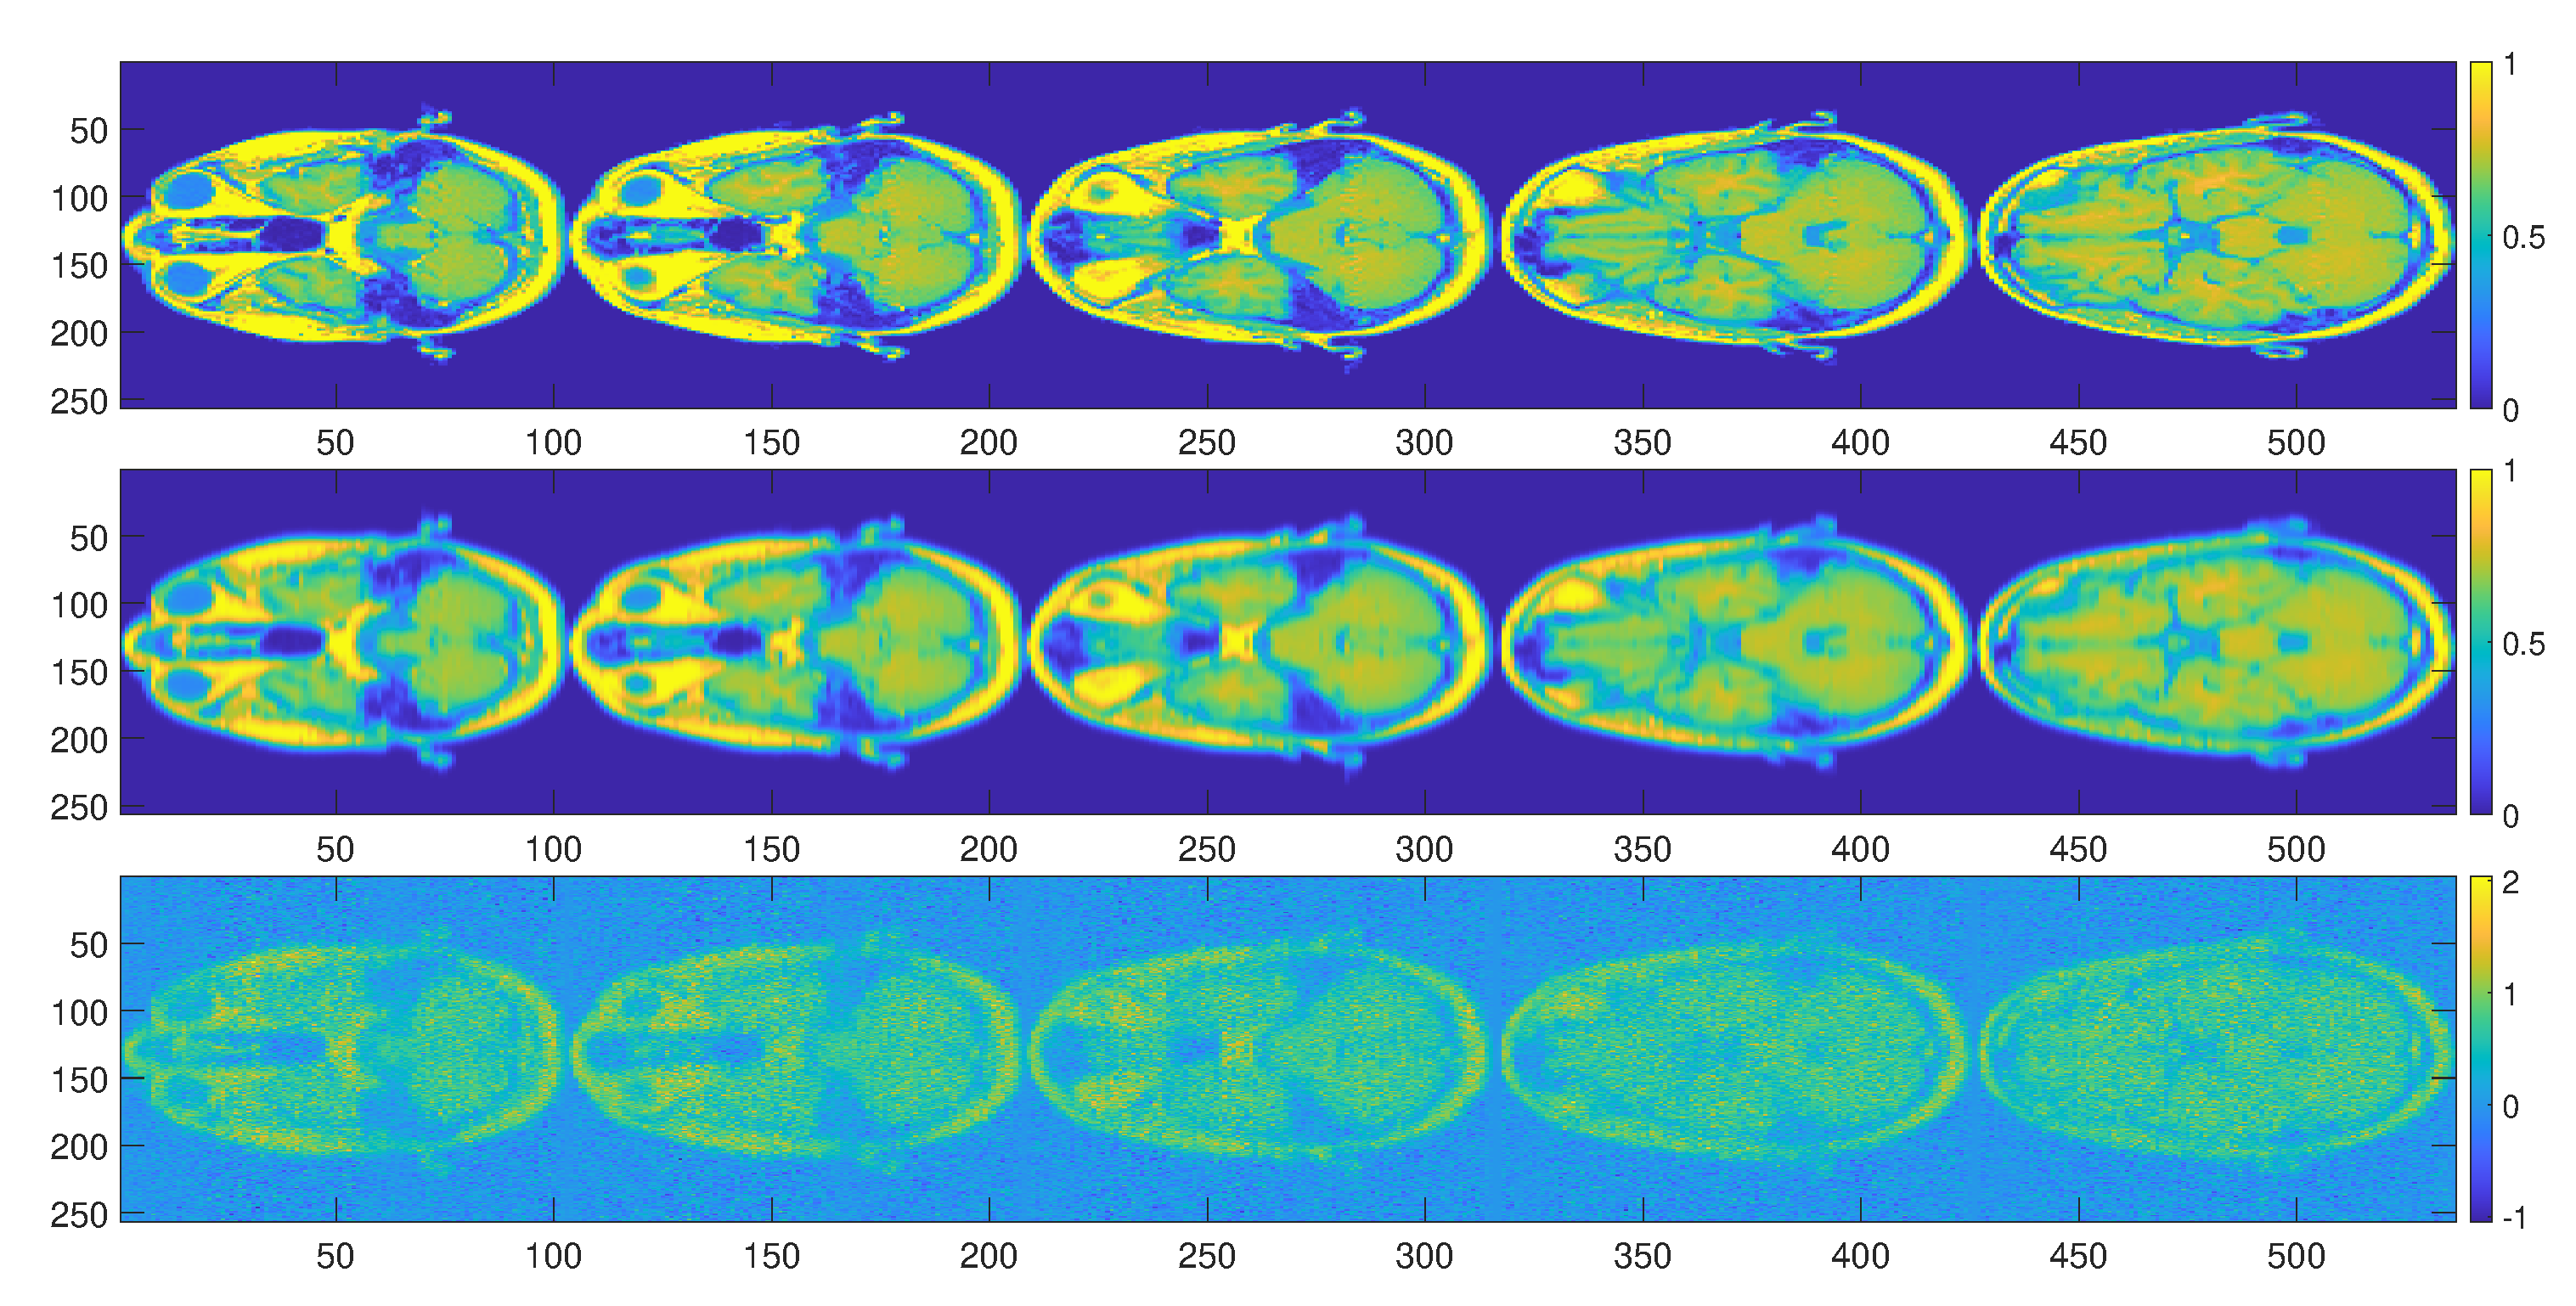
\includegraphics[scale=0.32]{Figures/Full_MRI_Data.eps}
\caption{MRI data formed by reformatting the MATLAB built-in MRI data. Each vector was blurred using a Gaussian kernel and normal noise was added; the resulting vectors are shown at the bottom. The dimension of all three images is $256 \times 536$.}
\label{fig:MRI 1D}
\end{figure}

\noindent The other problem is two-dimensional that utilizes the images in Figure \ref{fig:MESSENGER True} of the planet Mercury obtained by the MESSENGER space probe. 

\begin{figure}[ht]
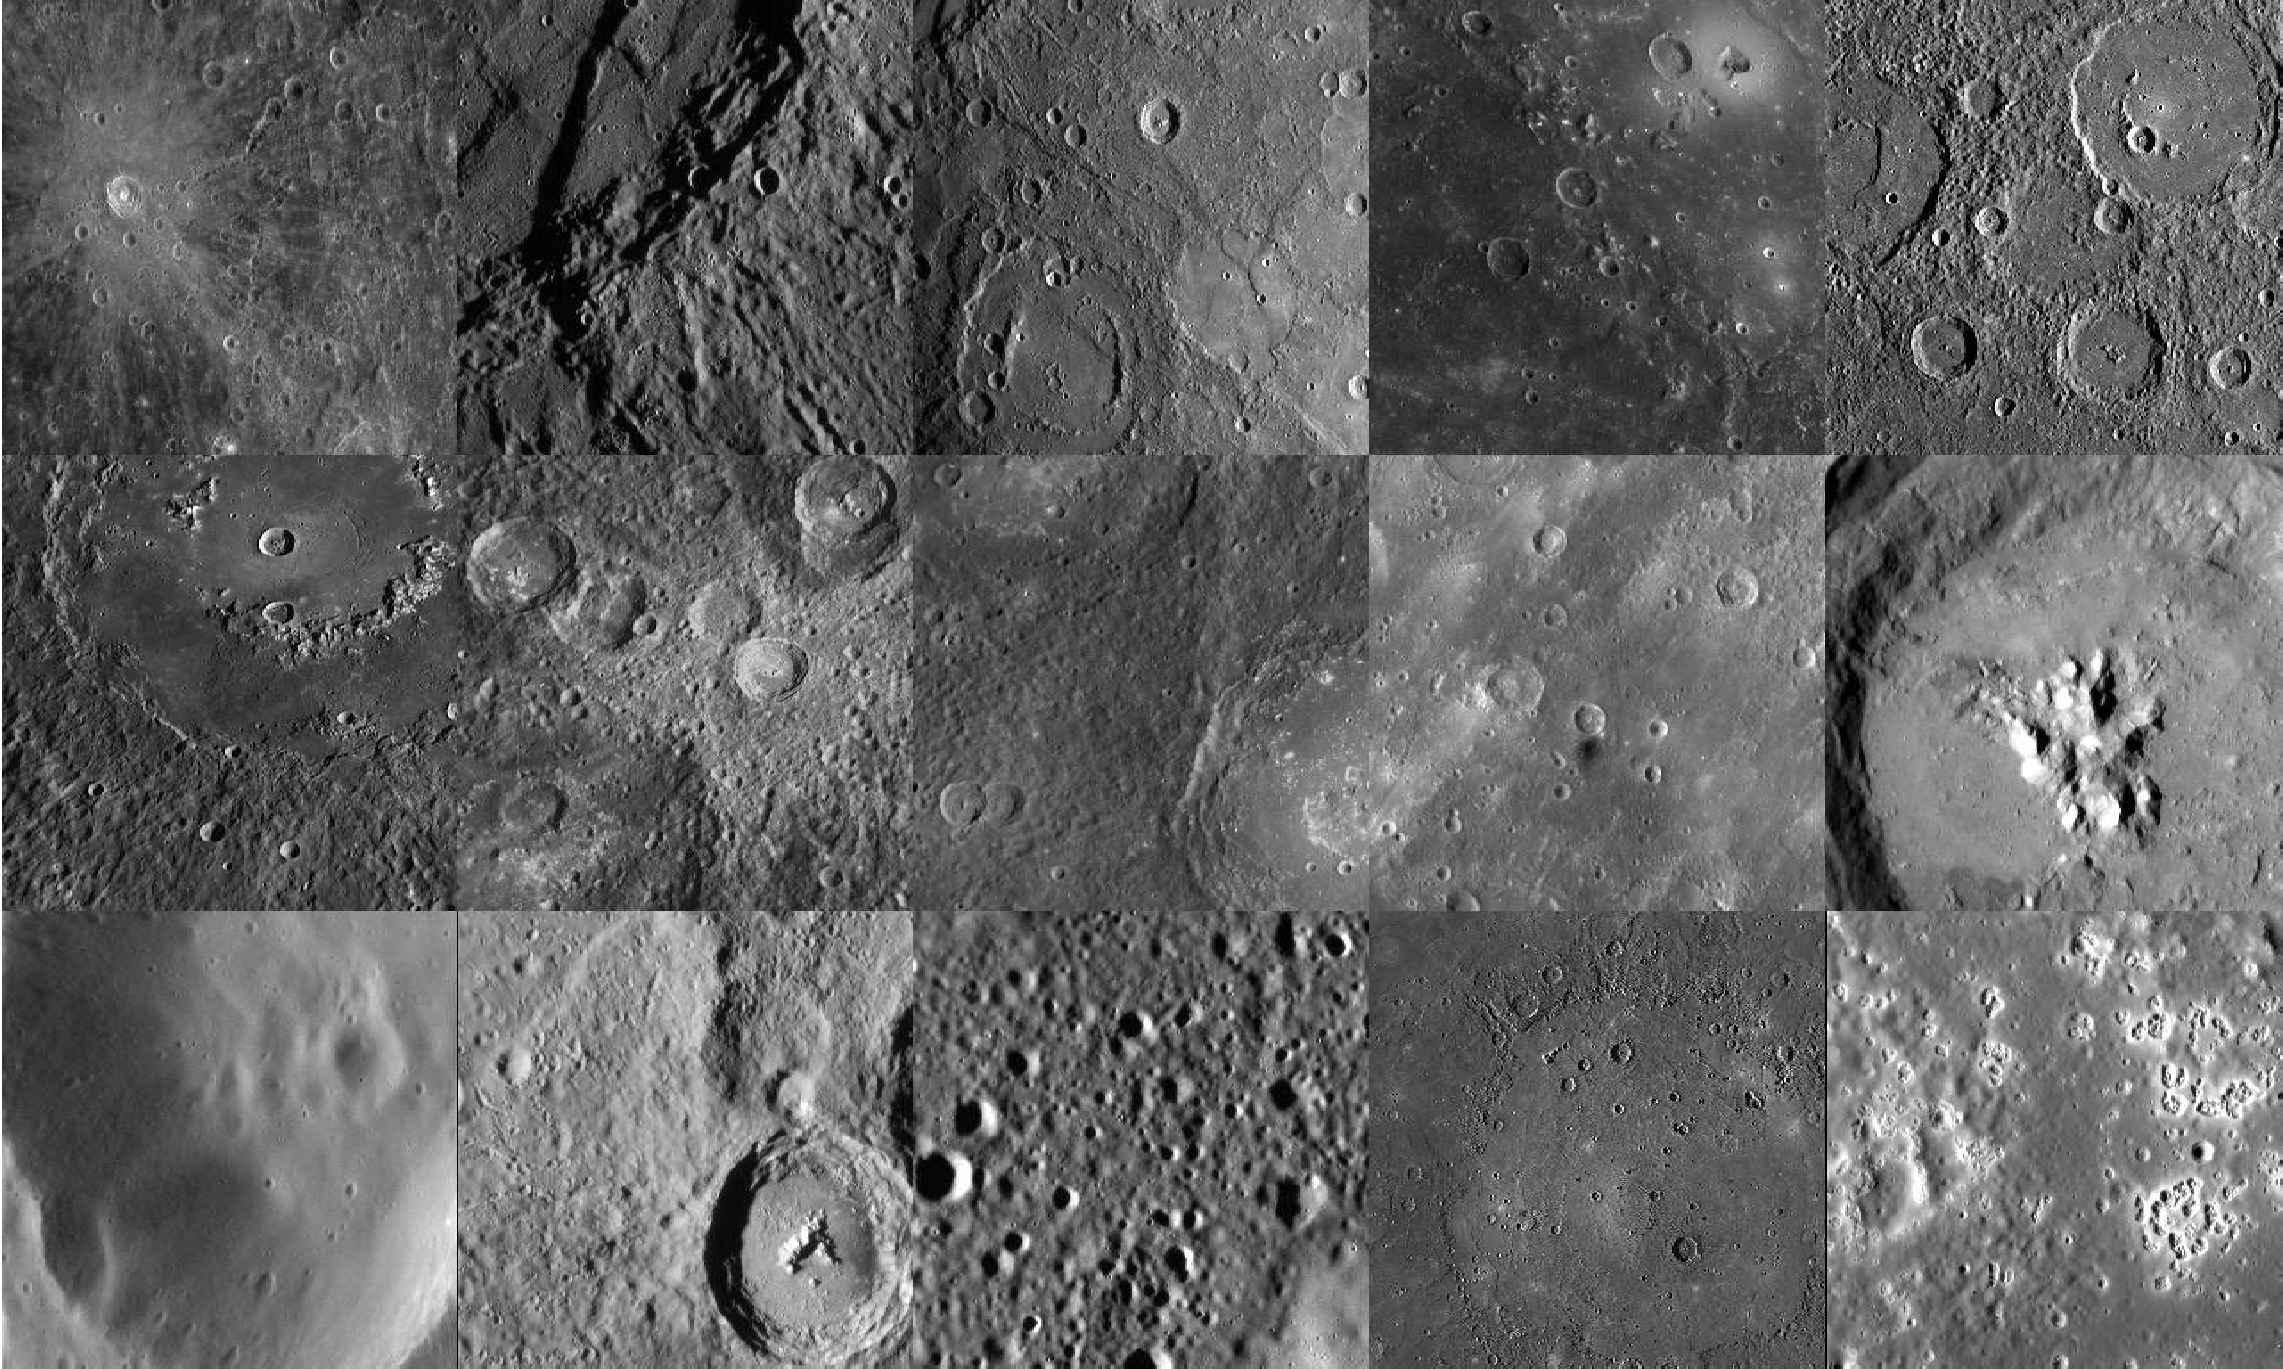
\includegraphics[scale=0.36]{Figures/MESSENGER}
\caption{Selected images used for MESSENGER two-dimensional test problem. Available courtesy of NASA/Johns  Hopkins  University  Applied  Physics  Laboratory/Carnegie Institution of Washington \cite{MESSENGER}.}
\label{fig:MESSENGER True}
\end{figure}

\noindent The MESSENGER images are available to the public courtesy of NASA, the Johns Hopkins University Applied Physics Laboratory, and the Carnegie Institution of Washington \cite{MESSENGER}. \par
For both problems, the following definition of signal-to-noise ratio (SNR) is used as a measurement for noise content in the images:
\begin{equation}
\label{eq:SNR}
\text{SNR} = 10\log_{10}\left(\frac{\mathcal{P}_{\text{signal}}}{\mathcal{P}_{\text{noise}}}\right).
\end{equation}
In the discrete setting, the average power $\mathcal{P}$ of a vector $\xVec$ of length $n$ is defined as $\frac{1}{\mA}\|\xVec\|^2_2$. Using this definition for vectors $\bVec$ and $\noiseVec$, $\mathcal{P}_{\text{signal}} = \frac{1}{\mA}\|\bVec\|^2_2$ and $\mathcal{P}_{\text{noise}} = \frac{1}{\mA}\|\noiseVec\|^2_2$ and so the quotient in the logarithm is $\|\bVec\|_2^2/\|\noiseVec\|_2^2$. If $\bVec$ is a matrix representing an image, in which case $\noiseVec$ is a realization of a random matrix, the 2-norms can be replaced by the Frobenius norm.

\subsection{One-dimensional problem} \label{sec:1D}
The one-dimensional test problem uses the MRI data built into MATLAB, which can be accessed by the command \texttt{load mri.mat}. Five horizontal slices were selected and reformatted as a single image (Figure \ref{fig:MRI 1D}) of dimensions $256 \times 536$. The default dimension of each horizontal MRI slice accessible using \texttt{load mri.mat} is $128 \times 128$. Linear interpolation was used to double the number of rows; the number of columns of the concatenated MRI slices was trimmed to to eliminate leading and trailing zero columns. The columns of the image were then multiplied by a symmetric Toeplitz matrix, approximating a Fredholm integral equation of the first kind with a zero centered Gaussian kernel of variance 1 (each pixel representing a unit square in the continuous problem). The resulting MRI image is vertically blurred; see Figure \ref{fig:MRI 1D}. SNR values were selected randomly between 6 and 7 for each blurred column, and realizations of normal noise with the corresponding variances were added to blurred columns. The first $536/2 = 268$ columns of Figure \ref{fig:MRI 1D} served as the training set, while the remaining 268 columns serve as a validation set.  The following $255 \times 256$ penalty matrix $L$ was used, which represents an approximation of a first derivative operator:
\[L = \begin{bmatrix}
-1 & 1 & &  \\
 & \ddots &  \ddots & \\
 & & -1 & 1 \\
\end{bmatrix}.\]
The resulting system matrix in \eqref{eq:TikSol3} has full column rank, and so applying the normal equations in terms of the GSVD results in unique solutions. \par 
Figure \ref{fig:Parameters 1D MRI} illustrates a comparison of the methods in terms of the regularization parameters $\regparam$ selected as the number of training vectors increases. 

\begin{figure}[ht]
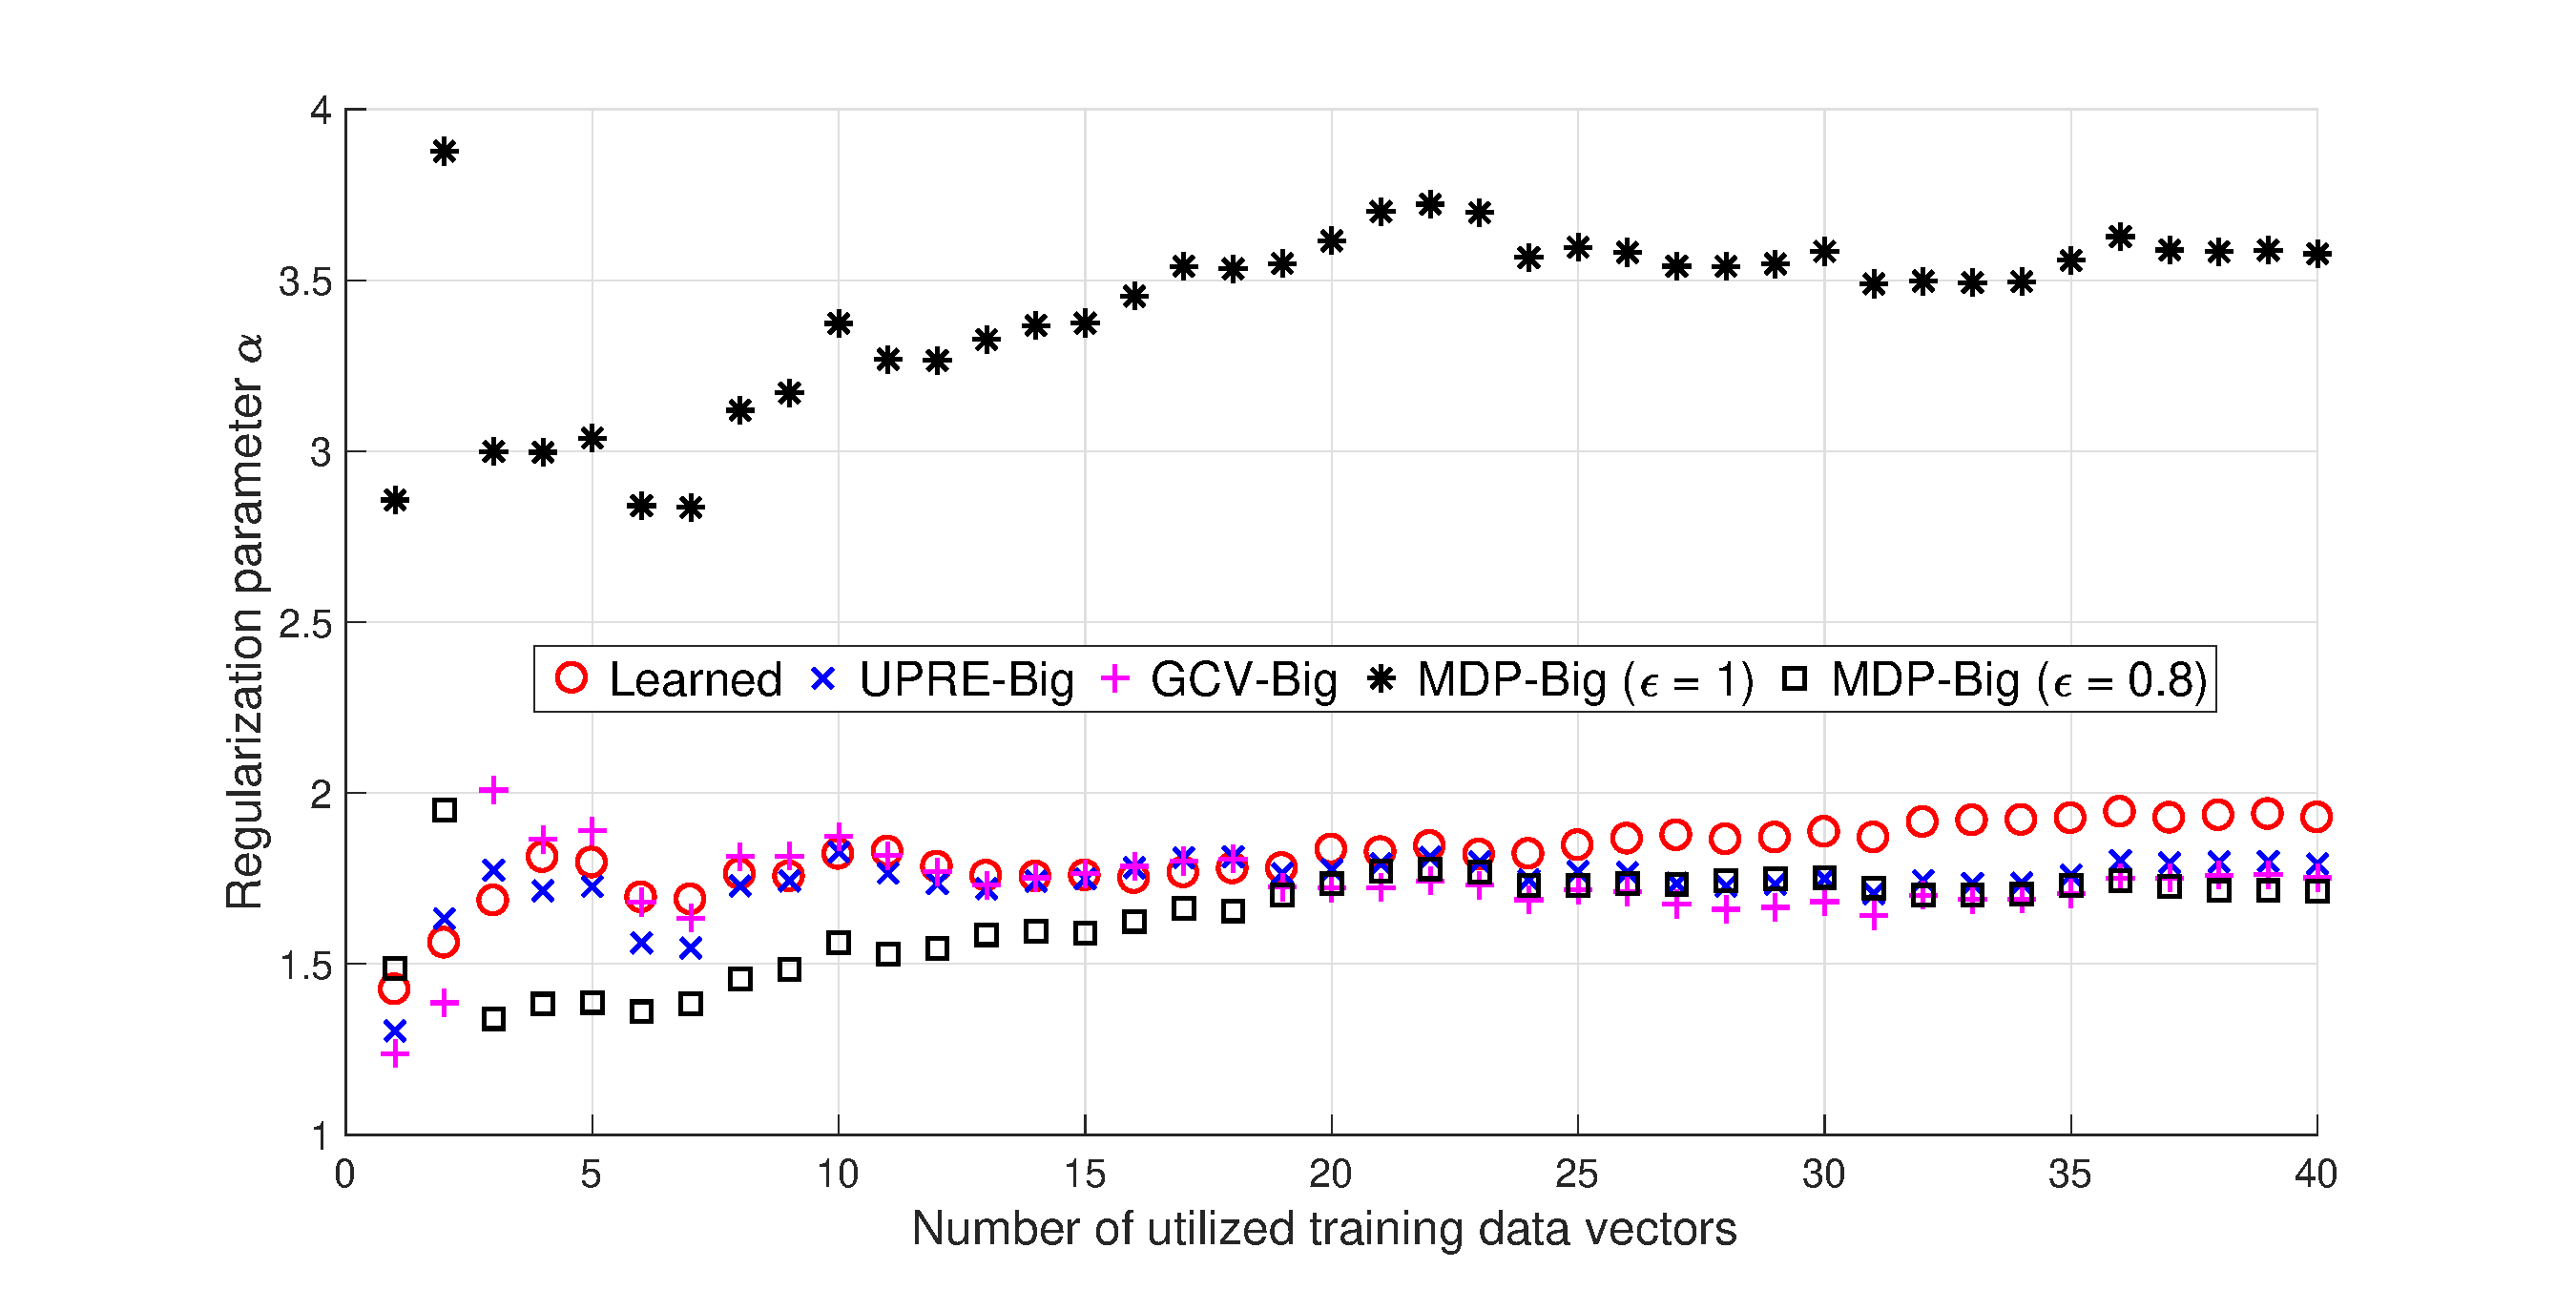
\includegraphics[scale=0.36]{Figures/Parameters1D_mri}
\caption{Trend of parameters selected by each adapted method as the number of training vectors increases. Note that the parameters essentially stabilize by about 40 training vectors out of the possible 268.}
\label{fig:Parameters 1D MRI}
\end{figure}

\noindent When the number of training vectors is small (e.g. between 1 and 10 from Figure \ref{fig:Parameters 1D MRI}), the parameters selected by all four methods change significantly. This can be attributed to the fact that all of the methods select a parameter that is either a root or a minimum of an average of functions. For a small amount of training vectors, each additional vector has more influence over the behavior of the adapted function. The parameters do seem to stabilize as the number of training vectors reach a certain point; in the problem being considered here, the parameters stabilize by about 40 training sets. The stabilization of the parameter most likely follows from the fact that each vector is part of the same type of image (MRI). It would seem unreasonable to expect the same stabilization when using vectors pulled from dissimilar images. \par 
Before looking at the relative errors of the regularized solutions, another observation regarding Figure \ref{fig:Parameters 1D MRI} can be made. While the parameters selected using the learning function \eqref{eq:Learning function} and the adapted UPRE and GCV methods are close (the maximum difference in the parameters does not exceed 0.5), the adapted MDP method consistently selected significantly larger parameters. A direct consequence is that the regularized solutions have higher relative errors. \par
Figure \ref{fig:Errors 1D MRI} shows the relative errors of the regularized solutions corresponding to the parameters from each method. 

\begin{figure}[ht]
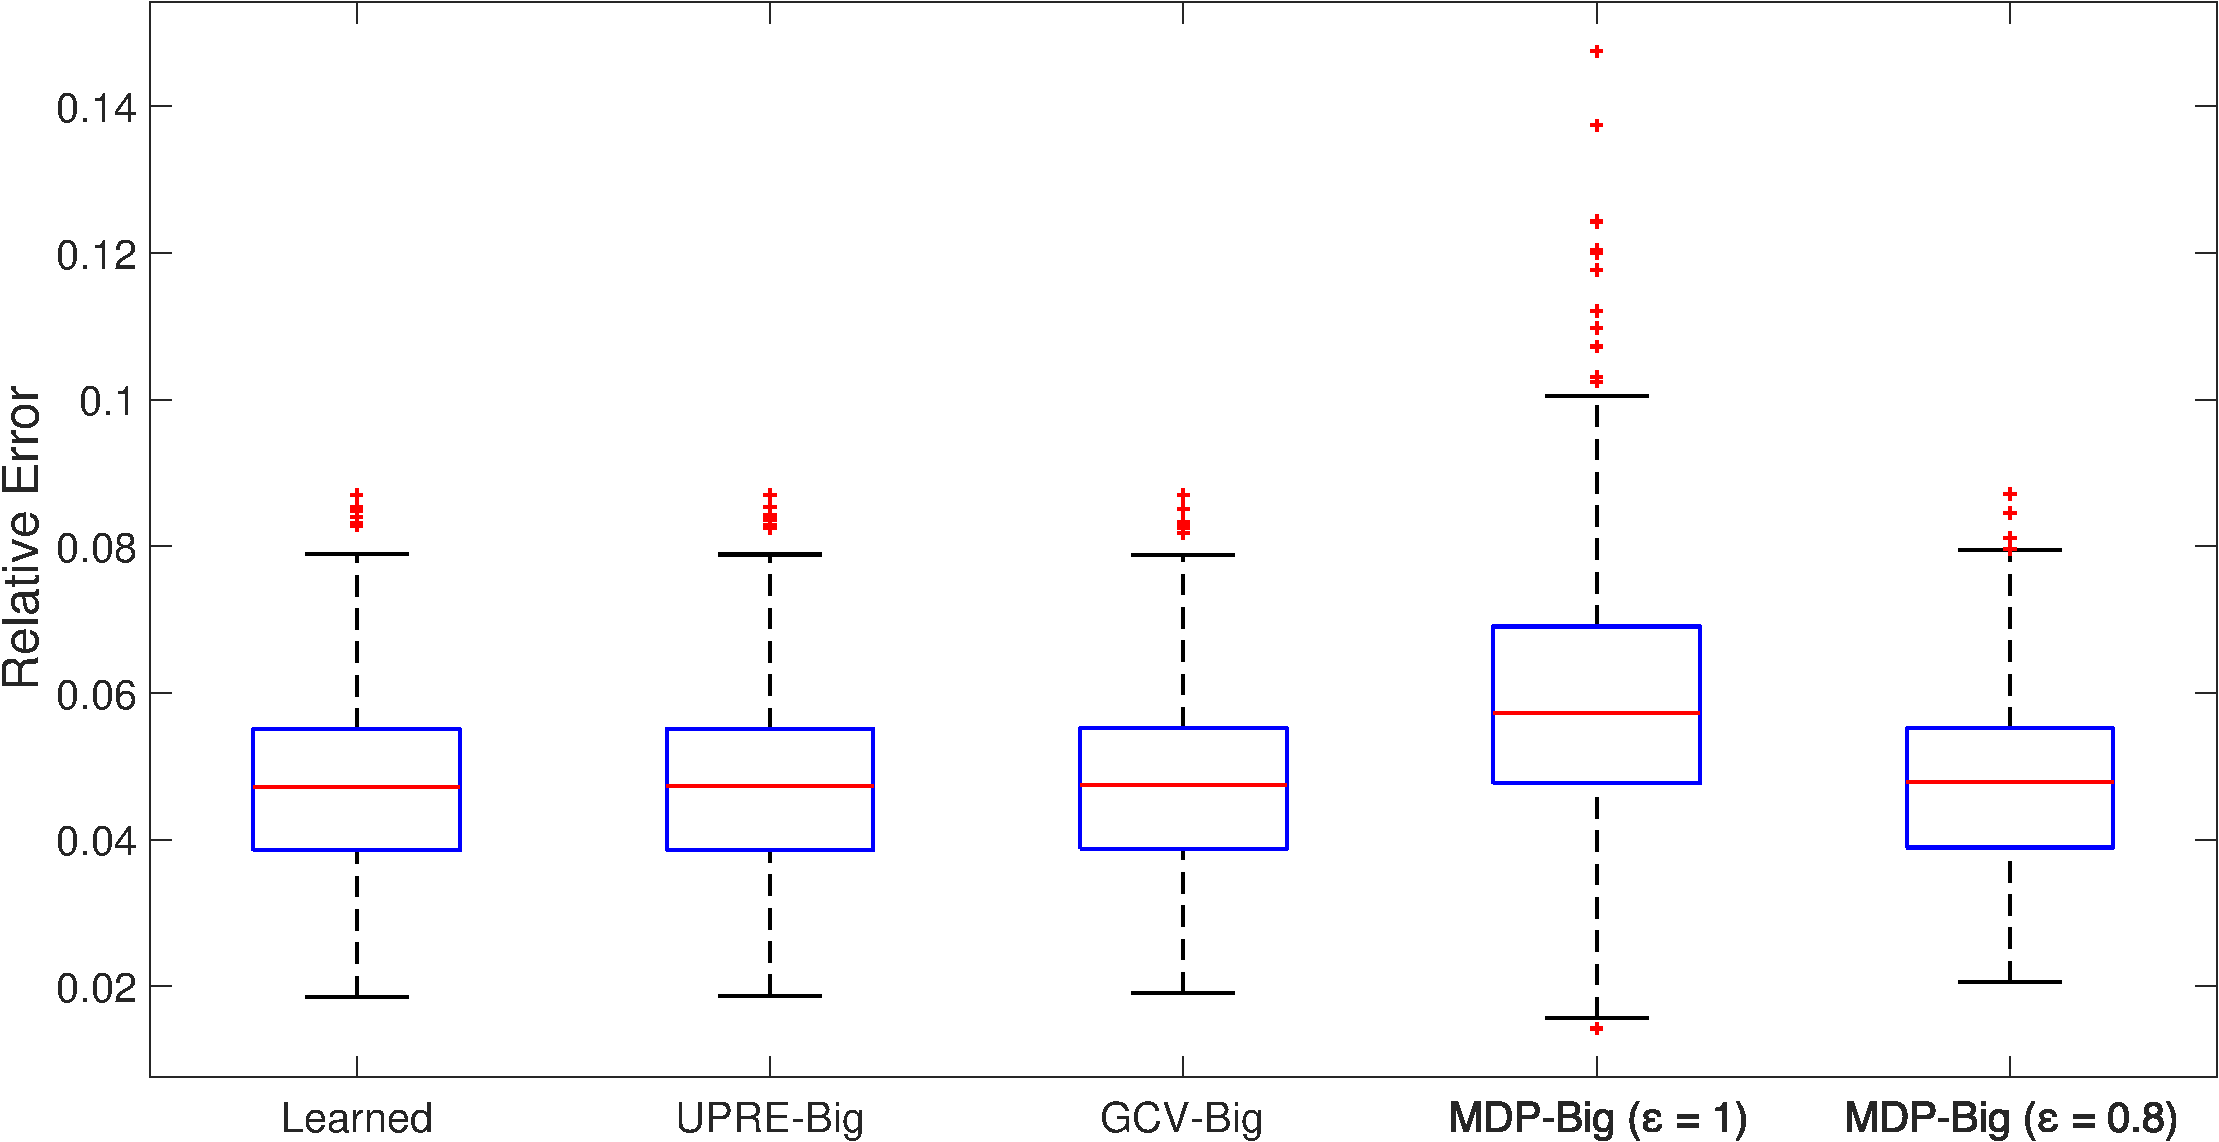
\includegraphics[scale=0.36]{Figures/Errors1D_mri}
\caption{Boxplots of the relative errors of each regularized solution versus the validation set. A parameter was selected using the full training set for each method, and the parameters of each method were used to generate regularized solutions from the validation set.}
\label{fig:Errors 1D MRI}
\end{figure}

\noindent Instead of using a relatively small amount of training vectors, like 40 out of 268 in Figure \ref{fig:Parameters 1D MRI}, the full training set was used to select a parameter from each method. These four parameters were then used to generate a regularized solution for each vector in the validation set, and the relative errors were computed against the true solutions. First, the relative errors obtained by the learning method and adapted UPRE and GCV methods are quite similar; the means of the relative errors are close, and there is a collection of upper outliers. In contrast, the adapted MDP method has a slightly larger mean relative error. However, the most striking visual characteristic from Figure \ref{fig:Errors 1D MRI} is the number of outliers in the MDP relative errors. The largest relative error obtained using the adapted MDP method is about twice the largest relative error of the other three methods. \par 
The one-dimensional test problem demonstrates that the adapted methods have potential for selecting viable regularization parameters that can be applied to multiple sets of data. The adapted UPRE and GCV performed competitively against the learning method, which relies on knowledge of the true training solutions. As stated previously, the success of the adapted methods is predicated on the similarity of the data sets being considered. However, this is not an unreasonable condition because data from a given experiment would hopefully vary little without significant change in the experimental set-up.

\subsection{Two-dimensional problems} \label{sec:2D}

The data sets of the two-dimensional test problem consist of images of size $256 \times 256$. A total of 16 images were used and split into training and validation sets containing eight images each. To obtain the 16 images from the $512 \times 512$ Mercury images in Figure \ref{fig:MESSENGER True}, eight images were randomly chosen and two $256 \times 256$ subimages of each image were randomly selected. The 16 images were then shuffled and split into training and validation sets. Another validation set of images, shown in Figure , was used that consisted of built-in MATLAB images.

\begin{figure}[ht]
\includegraphics[scale=0.36]{Figures/Validation Set 2}
\caption{The second validation set, consisting of built-in MATLAB images. From left to right starting in the top row, the images are: \texttt{rice.png}, \texttt{AT3\_1m4\_01.tif}, \texttt{circuit.tif}, \texttt{cameraman.tif}, \texttt{liftingbody.png}, \texttt{westconcordorthophoto.png}, \texttt{parkavenue.jpg}, and \texttt{llama.jpg}.}
\label{fig:Validation Set 2}
\end{figure}

A $256 \times 256$ point spread function (PSF) was formed using a discretization of the zero centered, circularly symmetric Gaussian kernel
\[k(x,y) = \exp\left(-\frac{(x^2 + y^2)}{2\nu}\right).\]
The parameter $\nu$ controls the width of the Gaussian kernel. Choosing $k(x,y)$ to be circularly symmetric is for convenience; a Gaussian kernel with different width parameters for the $x$ and $y$ directions can still be used to construct a PSF that is doubly symmetric for diagonalization via the DCT \cite{HansenNagyOLeary}. The two values of $\nu$ considered were 100 and 200. The corresponding PSFs were discretely convolved with each image as a means of blurring. SNR values of 25 and 40 were used to construct realizations of normal noise that were added to the blurred images for create the data. \par 
From this construction, the DCT was the primary tool for the 2D test problem as opposed to the GSVD. To ensure simultaneous diagonalization of the block system matrices $A$ and $L$, reflective boundary conditions were assumed so that both $A$ and $L$ have the same block structure. This special block structure is called BTTB + BTHB + BHTB + BHHB in \cite{HansenNagyOLeary}, with the ``T" and ``H" standing for Toeplitz and Hankel, respectively. One penalty matrix $L$ considered was the appropriately structured version of the discrete negative Laplacian operator, which is an approximation of the continuous Laplacian operator \cite{DebnathMikusinski2005,LeVeque2007}. The second penalty matrix was the identity. The structure of $A$ and $L$ allows for simultaneous diagonalization using two-dimensional DCT for numerical efficiency. \par 

\subsection{Multiparameter regularization}

\subsubsection{Two-dimensional problems}

\section{Conclusions and future work} \label{sec:Conclusion}
In conclusion, this paper demonstrate a means by which UPRE, MDP, and GCV methods can be extended to accommodate multiple data sets. The most general forms of functions associate with these methods are \eqref{eq:UPRE 3}, \eqref{eq:Big MDP}, \eqref{eq:GCV Big}, and , respectively. The adapted UPRE and MDP methods are novel in that their corresponding functions can be written as an average of the individual functions associate with each data set. None of the three adapted methods require knowledge of true solutions unlike the machine learning approach defined by \eqref{eq:Learning function}, though the MRI test problems demonstrate that the adapted methods can perform competitively. \par
There are various directions of future investigation. Perhaps the most significant results could be obtained through approaches of determining the necessary number of data sets for a stabilization of selected parameters. Figure \ref{fig:Parameters 1D MRI} suggests that obtained parameters stabilize fairly fast in relation to the number of data sets incorporate into the method functions. Another direction of future work would be to use the adapted methods on data sets containing images of differing objects. The MRI images used here are all visualizations of a human brain; it would be interesting to see how these methods perform for drastically different data sets.

\bibliographystyle{siam}
\bibliography{Parameter-Estimation}

\end{document}
